\documentclass[a4paper,12pt]{book}
\usepackage{graphicx}
\usepackage[export]{adjustbox}
\usepackage{subcaption}
\graphicspath{{Pics/}}
\usepackage{charter}
\usepackage{fancyhdr}
\usepackage{enumerate}
\usepackage{enumitem}
\usepackage{siunitx}
\usepackage{amssymb}
\usepackage{longtable}
\usepackage{multicol}
\usepackage{multirow}
\usepackage{hhline}
\usepackage{parskip}
\setlength{\parskip}{6pt}
\usepackage{ragged2e}
\usepackage{geometry} %margin
\geometry{left=2.1cm,right=2.1cm,top=3cm,bottom=3cm}
\usepackage{setspace}
\SetSinglespace{1.2}
\singlespacing
\renewcommand{\ttfamily}{\fontfamily{pcr}\selectfont}
%\renewcommand{\familydefault}{\rmdefault}

\usepackage[,table]{xcolor}
\definecolor{LightBlue}{cmyk}{0.16,0.03,0.04,0}
\definecolor{Title}{cmyk}{0.8,0.1,0,0.3}
\setlength{\arrayrulewidth}{0.3mm}
\setlength{\tabcolsep}{2pt}
\setlength{\headheight}{15pt}
\renewcommand{\arraystretch}{1}
\usepackage{tikz}
\usepackage{nicematrix}
\newcommand*\circled[1]{\tikz[baseline=(char.base)]{\node[shape=circle,draw,inner sep=1pt] (char) {#1};}}

\newcolumntype{s}{>{\columncolor{Title}\RaggedLeft} m{3.5em}} % columntype for chapter title
\newcolumntype{d}{>{\columncolor{LightBlue}\RaggedRight} m{\textwidth}} % columntype for code bloc
\newcolumntype{a}{>{\columncolor{LightBlue}\RaggedRight} m{0.96\textwidth}} % columntype for secondary code bloc

\usepackage{titlesec}
\usepackage[hidelinks]{hyperref}
\urlstyle{same}

\captionsetup[figure]{labelsep=period,font={bf}}
\captionsetup[table]{font={bf},labelsep=period}

\newcommand{\titlename}{}

\newcommand{\chaptertitle}[2]{ %reset chapter format
\vspace{-120pt}
\gdef\titlename{#1}
{
\SetSinglespace{1.1}
\singlespacing
\Huge\bfseries
\setlength{\tabcolsep}{8pt}
\renewcommand{\arraystretch}{1.5}
\begin{tabular}{s >{\RaggedRight}m{14.5em}}
\textcolor{white}{Chapter\newline\thechapter}&\textcolor{Title}{#2}
\end{tabular}
}
}

\newcommand{\partpic}[1]{%insert picture
    \tikz[remember picture,overlay] \node at (current page.center){\includegraphics[width=\paperwidth]{#1}};
}

\titleformat{\part} %reset part %format
{\huge\bfseries} % format
{} % label
{0em} % sep
{\Centering} % before-code

\titleformat{\chapter} %reset chapter %format
{\huge\bfseries} % format
{} % label
{0em} % sep
{\Centering} % before-code
\titlespacing{\chapter}{0pt}{0pt}{0pt}

\titleformat{\section} %reset section %format
{\Large\bfseries} % format
{\textcolor{Title}{\thesection}} % label
{0.5em} % sep
{\color{Title}} % before-code
\titlespacing{\section}{0pt}{12pt}{6pt}

\titleformat{\subsection} %reset subsection %format
{\large\bfseries} % format
{\textcolor{Title}{\thesubsection}} % label
{0.5em} % sep
{\color{Title}} % before-code
\titlespacing{\subsection}{0pt}{8pt}{6pt}

\newenvironment{term}[1]{
    \textbf{#1}

    \leftskip 1em
    \parskip 0pt
}

\newenvironment{secterm}[1]{
    \textbf{#1}

    \leftskip 2em
    \parskip 0pt
}

\newenvironment{codebloc}{ %define code bloc style
    \ttfamily\footnotesize
    \renewcommand{\arraystretch}{1}
}

\newcommand{\note}[2][NOTE]{ %Note/Tips
\vspace{6pt}
\begin{tabular}{b{\textwidth}}
\hline
\fontfamily{phv}\selectfont \textbf{#1}\\
\leftskip 1em #2\\
\hline
\end{tabular}
}

\newcommand{\secnote}[2][NOTE]{ %Note/Tips
\vspace{6pt}
\begin{tabular}{b{0.93\textwidth}}
\hline
\fontfamily{phv}\selectfont \textbf{#1}\\
\leftskip 1em #2\\
\hline
\end{tabular}
}

\title{ESP32-C3 Wireless Adventure\par \Large A comprehensive guide to IoT}
\author{Espressif Systems}
\date{\today}

\pagestyle{fancy} % reset head&foot
\fancyhead{} % clear all header fields
\renewcommand\headrulewidth{0pt}
\fancyfoot{} % clear all footer fields
\setcounter{chapter}{3}

\begin{document}

\fancyfoot[LE]{\fontfamily{cmss}\selectfont{\textbf{\thepage} \ \textit{ESP32-C3 Wireless Adventure: A comprehensive guide to IoT}}}
\fancyfoot[RO]{\fontfamily{cmss}\selectfont{\textit{Chapter \thechapter. \titlename} \ \textbf{\thepage}}}

\chapter[Setting Up Development Environment]{\chaptertitle{Setting Up Development Environment}{Setting Up\newline Development Environment}}

\vspace{36pt}
This chapter focuses on ESP-IDF, the official software development framework for ESP32-C3. We’ll explain how to set up the environment on various operating systems, and introduce the project structure and build system of ESP-IDF, as well as the usage of related development tools. Then we’ll present the compiling and running process of an example project, while offering a detailed explanation of the output log at each stage.

\section{ESP-IDF Overview}
ESP-IDF (Espressif IoT Development Framework) is a one-stop IoT development framework provided by Espressif Technology. It uses C/C++ as the main development language and supports cross-compilation under mainstream operating systems such as Linux, Mac, and Windows. The example programs included in this book are developed using ESP-IDF, which offers the following features:

\begin{itemize}[leftmargin=1.5em]
    \item \textbf{SoC system-level drivers}. ESP-IDF includes drivers for ESP32, ESP32-S2, ESP32-C3, and other chips. These drivers encompass peripheral low level (LL) library, hardware abstraction layer (HAL) library, RTOS support and upper-layer driver software, etc.
    \item \textbf{Essential components}. ESP-IDF incorporates fundamental components required for IoT development. This includes multiple network protocol stacks such as HTTP and MQTT, a power management framework with dynamic frequency modulation, and features like Flash Encryption and Secure Boot, etc.
    \item \textbf{Development and production tools}. ESP-IDF provides commonly used tools for building, flash, and debugging during development and mass production (see Figure \ref{Building, flashing, and debugging tools for development and mass production}), such as the building system based on CMake, the cross-compilation tool chain based on GCC, and the JTAG debugging tool based on OpenOCD, etc.
\end{itemize}

\begin{figure}[h!]
    \centering
    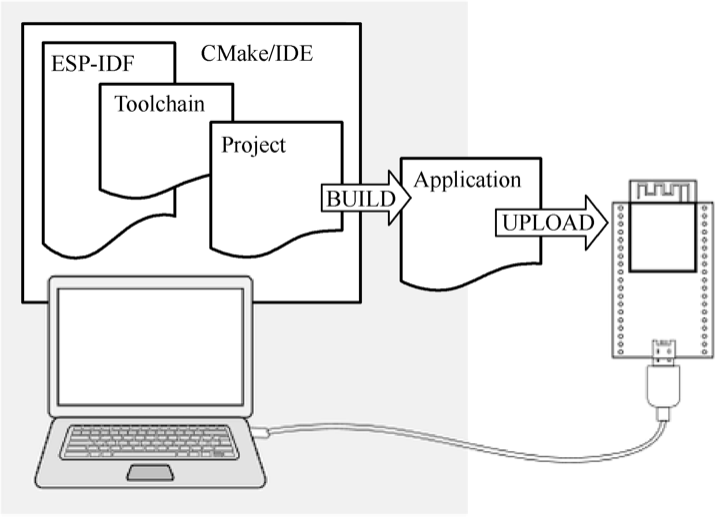
\includegraphics[width=0.6\textwidth]{D4Z/4-1}
    \caption{\Centering Building, flashing, and debugging tools for development and mass production}
    \label{Building, flashing, and debugging tools for development and mass production}
\end{figure}

It is worth noting that the ESP-IDF code primarily adheres to the the Apache 2.0 open-source license. Users can develop personal or commercial software without restrictions while complying with the terms of the open-source license. Additionally, users are granted permanent patent licenses free of charge, without the obligation to open-source any modifications made to the source code.

\subsection{ESP-IDF Versions}
The ESP-IDF code is hosted on GitHub as an open-source project. Currently, there are three major versions available: v3, v4, and v5. Each major version usually contains various sub-versions, such as v4.2, v4.3, and so on. Espressif Systems ensures a 30-month support for bug fixes and security patches for each released sub-version. Therefore, revisions of sub-versions are also released regularly, such as v4.3.1, v4.2.2, etc. Table 4.1 shows the support status of different ESP-IDF versions for Espressif chips, indicating whether they are in a preview stage (offering support for preview versions, which may lack certain features or documentation) or are officially supported.

\begin{table}[h!]
    \renewcommand{\arraystretch}{1.5}
    \caption{Support status of different ESP-IDF versions for Espressif chips}
    \begin{tabular}{|>{\Centering}m{5.5em}|>{\Centering}m{6.3em}|>{\Centering}m{6.3em}|>{\Centering}m{6.3em}|>{\Centering}m{6.3em}|>{\Centering}m{6.3em}|}
        \hline
        \rowcolor{LightBlue} \textbf{Series}&\textbf{v4.1}&\textbf{v4.2}&\textbf{v4.3}&\textbf{v4.4}&\textbf{v5.0}\\
        \hline
        ESP32&supported&supported&supported&supported&supported\\
        \hline
        ESP32-S2&&supported&supported&supported&supported\\
        \hline
        ESP32-C3&&&supported&supported&supported\\
        \hline
        ESP32-S3&&&&supported&supported\\
        \hline
        ESP32-C2&&&&&supported\\
        \hline
        ESP32-H2&&&&preview&preview\\
        \hline
    \end{tabular}
\end{table}

The iteration of major versions often involves adjustments to the framework structure and updates to the compilation system. For example, the major change from v3.* to v4.* was the gradual migration of the build system from Make to CMake. On the other hand, iteration of minor versions typically entails the addition of new features or support for new chips.

It is important to distinguish and understand the relationship between stable versions and GitHub branches. Versions labeled as v*.* or v*.*.* represent stable versions that have passed complete internal testing by Espressif. Once fixed, the code, tool chain, and release documents for the same version remain unchanged. However, GitHub branches (e.g., the \verb|release/v4.3| branch) undergo frequent code commits, often on a daily basis. Therefore, two code snippets under the same branch may differ, necessitating developers to promptly update their code accordingly.

\subsection{ESP-IDF Git Workflow}

Espressif follows a specific Git workflow for ESP-IDF, outlined as follows:

\begin{itemize}[leftmargin=1.5em]
    \item New changes are made on the \verb|master| branch, which serves as the main development branch. The ESP-IDF version on the \verb|master| branch always carries a \verb|-dev| tag to indicate that it is currently under development, such as \verb|v4.3-dev|. Changes on the \verb|master| branch will first be reviewed and tested in Espressif’s internal repository, and then pushed to GitHub after automated testing is complete.
    \item Once a new version has completed feature development on the \verb|master| branch and met the criteria for entering beta testing, it transitions to a new branch, such as \verb|release/|\\ \verb|v4.3|. In addition, this new branch is tagged as a pre-release version, like \verb|v4.3-beta1|. Developers can refer to the GitHub platform to access the complete list of branches and tags for ESP-IDF. It’s important to note that the beta version (pre-release version) may still have a significant number of known issues. As the beta version undergoes continuous testing, bug fixes are added to both this version and the \verb|master| branch simultaneously. Meanwhile, the \verb|master| branch may have already begun developing new features for the next version. When testing is nearly complete, a release candidate (\verb|rc|) label is added to the branch, indicating that it is a potential candidate for the official release, such as \verb|v4.3-rc1|. At this stage, the branch remains a pre-release version.
    \item If no major bugs are discovered or reported, the pre-release version eventually receives a major version label (e.g., v5.0) or a minor version label (e.g., v4.3) and becomes an official release version, which is documented in the release notes page. Subsequently, any bugs identified in this version are fixed on the release branch. After manual testing is completed, the branch is assigned a bug-fix version label (e.g., v4.3.2), which is also reflected on the release notes page.
\end{itemize}

\subsection{Choosing a Suitable Version}
Since ESP-IDF officially began supporting ESP32-C3 from version v4.3, and v4.4 has not yet been officially released at the time of writing this book, the version used in this book is v4.3.2, which is a revised version of v4.3. However, it is important to note that by the time you read this book, v4.4 or newer versions may already be available. When selecting a version, we recommend the following:

\begin{itemize}[leftmargin=1.5em]
    \item For \textbf{entry-level developers}, it is advisable to choose the stable v4.3 version or its revised version, which aligns with the example version used in this book.
    \item For \textbf{mass production} purposes, it is recommended to use the latest stable version to to benefit from the most up-to-date technical support.
    \item If you intend to experiment with \textbf{new chips} or explore \textbf{new product features}, please use the \verb|master| branch. The latest version contains all the latest features, but keep in mind that there may be known or unknown bugs present.
    \item If the stable version being used does not include the desired new features and you wish to \textbf{minimise the risks} associated with the \verb|master| branch, consider using the corresponding release branch, such as the \verb|release/v4.4| branch. Espressif’s GitHub repository will first create the \verb|release/v4.4| branch and subsequently release the stable v4.4 version based on a specific historical snapshot of this branch, after completing all feature development and testing.
\end{itemize}

\subsection{Overview of ESP-IDF SDK Directory}
The ESP-IDF SDK consists of two main directories: \verb|esp-idf| and \verb|.espressif|. The former contains ESP-IDF repository’s source code files and compilation scripts, while the latter mainly stores compilation tool chains and other software. Familiarity with these two directories will help developers make better use of available resources and speed up the development process. The directory structure of ESP-IDF is described below:

\begin{enumerate}[label=(\arabic*),leftmargin=2em]
    \item \textbf{ESP-IDF repository code directory} (\texttt{$\sim$/esp/esp-idf}), as shown in Figure \ref{ESP-IDF repository code directory}.

    \begin{figure}[h!]
        \centering
        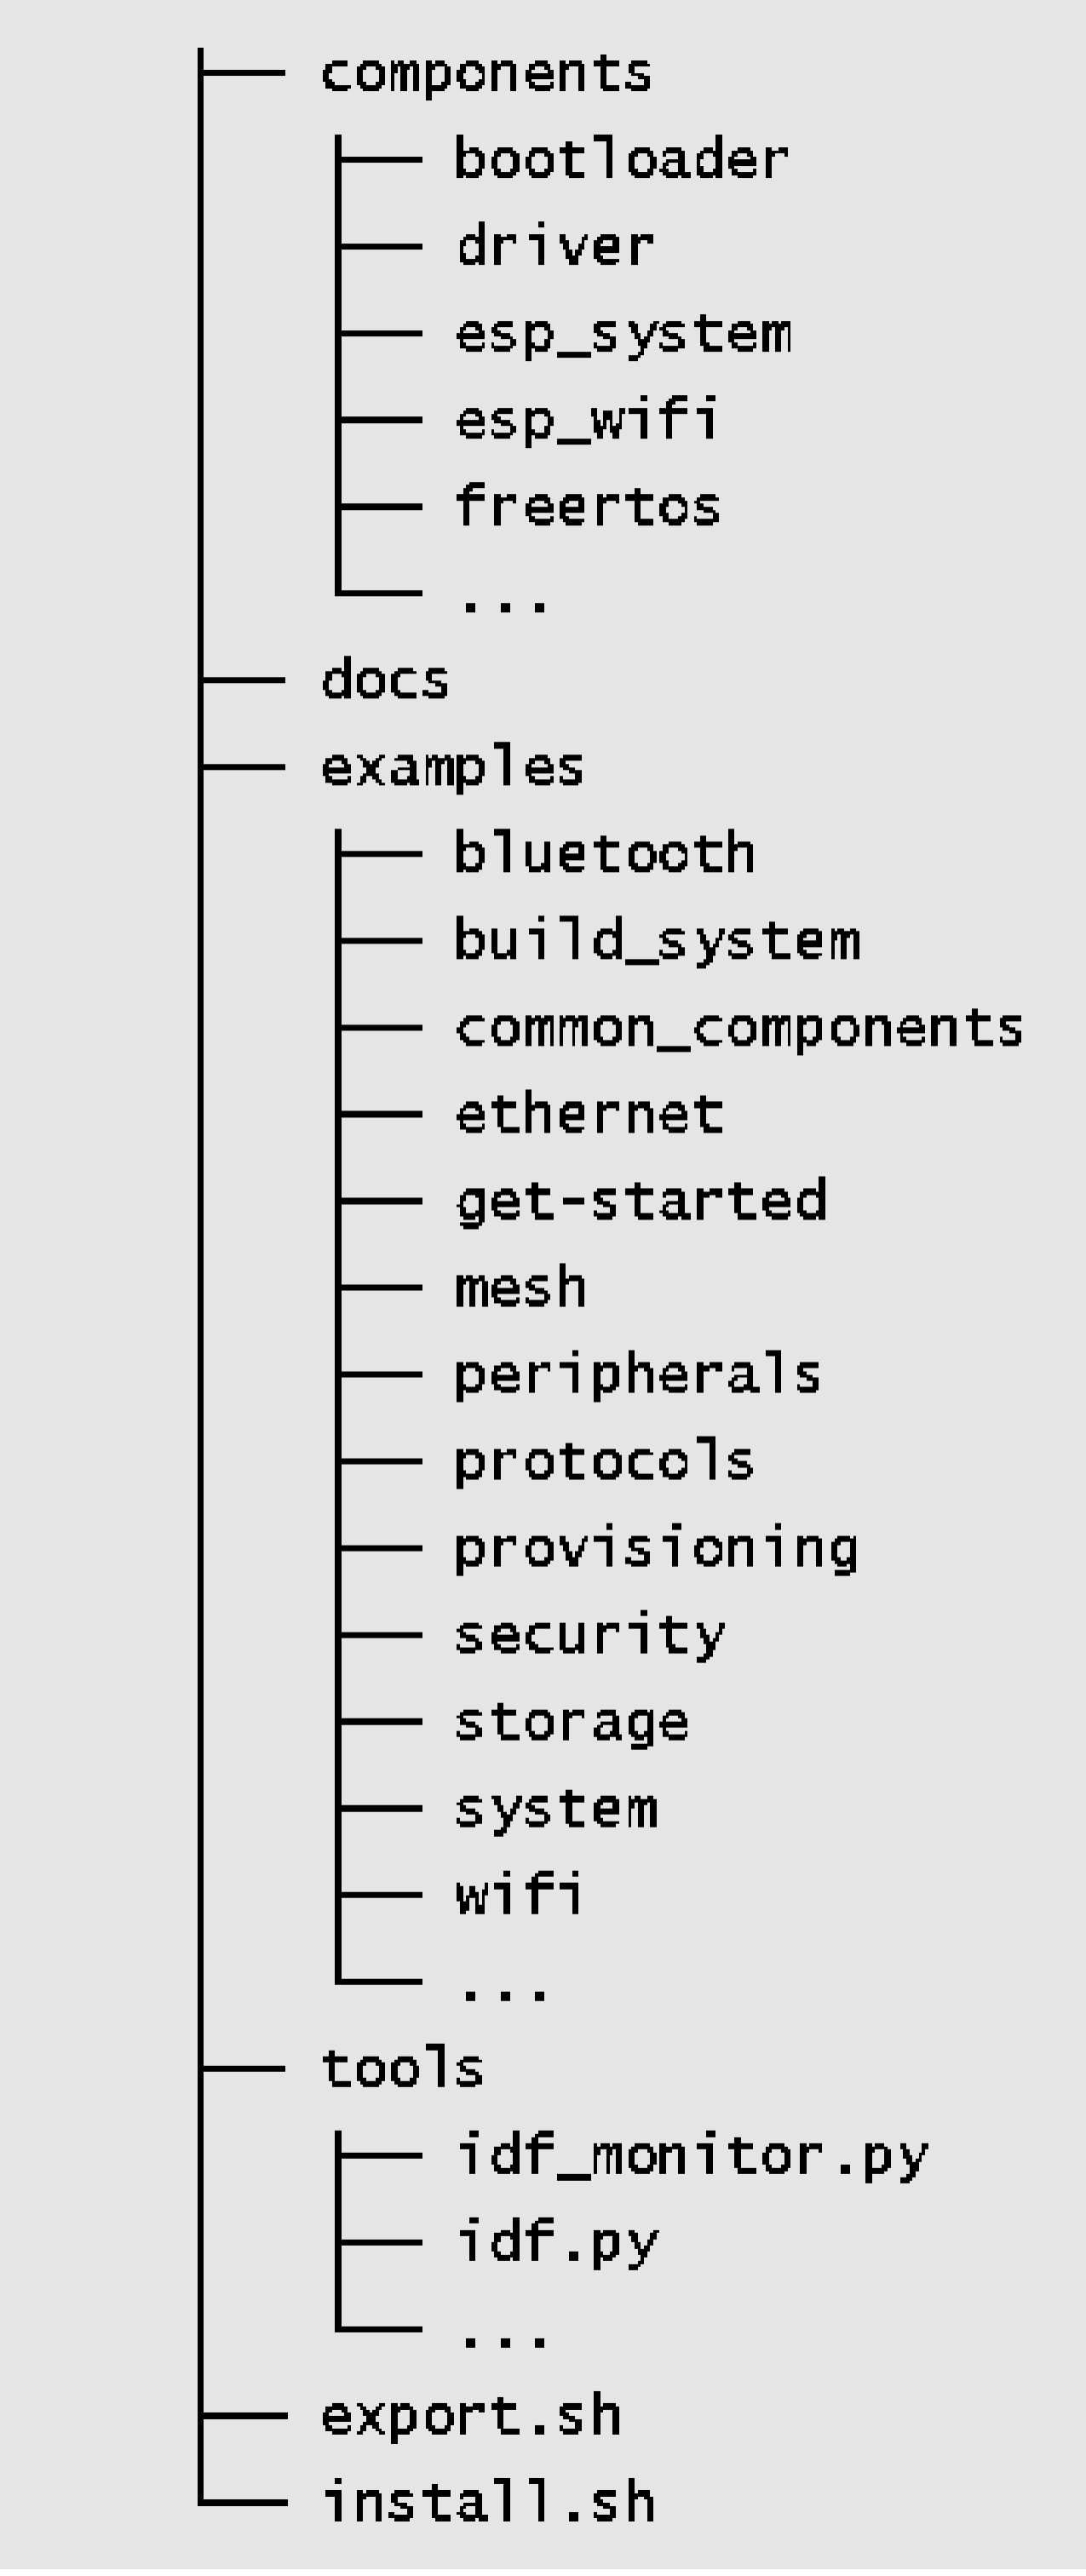
\includegraphics[width=0.35\textwidth]{D4Z/4-2}
        \caption{ESP-IDF repository code directory}
        \label{ESP-IDF repository code directory}
    \end{figure}

    \begin{enumerate}[label=\textbf{\alph*.},leftmargin=0em]
        \item \textbf{Component directory \texttt{components}}

        This core directory integrates numerous essential software components of ESP-IDF. No project code can be compiled without relying on the components within this directory. It includes driver support for various Espressif chips. From the LL library and HAL library interfaces for peripherals to the upper-level Driver and Virtual File System (VFS) layer support, developers can choose the appropriate components at different levels for their development needs. ESP-IDF also supports multiple standard network protocol stacks such as TCP/IP, HTTP, MQTT, WebSocket, etc. Developers can utilise familiar interfaces like Socket to build network applications. Components provide comprehensive functionality and can be easily integrated into applications, allowing developers to focus solely on the business logic. Some common components include:

        \begin{itemize}[leftmargin=1em]
            \item \verb|driver|: This component contains peripheral driver programs for various Espressif chip series, such as GPIO, I2C, SPI, UART, LEDC (PWM), etc. The peripheral driver programs in this component offer chip-independent abstract interfaces. Each peripheral has a common header file (such as \verb|gpio.h|), eliminating the need to deal with different chip-specific support questions.
            \item \verb|esp_wifi|: Wi-Fi, as a special peripheral, is treated as a separate component. It includes multiple APIs such as initialisation of various Wi-Fi driver modes, parameter configuration, and event processing. Certain functions of this component are provided in the form of static link libraries. ESP-IDF also provides comprehensive driver documentation for ease of use.
            \item \verb|freertos|: This component contains the complete FreeRTOS code. Apart from providing comprehensive support for this operating system, Espressif has also extended its support to dual-core chips. For dual-core chips like ESP32 and ESP32-S3, users can create tasks on specific cores.
        \end{itemize}

        \item \textbf{Document directory \texttt{docs}}

        This directory contains ESP-IDF related development documents, including the Get Started Guide, API Reference Manual, Development Guide, etc.

        \secnote{After being compiled by automated tools, the contents of this directory are deployed at \url{https://docs.espressif.com/projects/esp-idf}. Please ensure to switch the document target to ESP32-C3 and select the specified ESP-IDF version.}

        \item \textbf{Script tool \texttt{tools}}

        This directory contains commonly used compilation front-end tools such as \verb|idf.py|, and the monitor terminal tool \verb|idf_monitor.py|, etc. The sub-directory \verb|cmake| also contains core script files of the compilation system, serving as the foundation for implementing ESP-IDF compilation rules. When adding the environment variables, the contents within the \verb|tools| directory are added to the system environment variable, allowing \verb|idf.py| to be executed directly under the project path.

        \item \textbf{Example program directory \texttt{examples}}

        This directory comprises a vast collection of ESP-IDF example programs that demonstrate the usage of component APIs. The examples are organised into various sub-directories based on their categories:

        \begin{itemize}[leftmargin=1em]
            \item \verb|get-started|: This sub-directory includes entry-level examples like “hello world” and “blink” to help users grasp the basics.
            \item \verb|bluetooth|: You can find Bluetooth related examples here, including Bluetooth LE Mesh, Bluetooth LE HID, BluFi, and more.
            \item \verb|wifi|: This sub-directory focuses on Wi-Fi examples, including basic programs like Wi-Fi SoftAP, Wi-Fi Station, \verb|espnow|, as well as proprietary communication protocol examples from Espressif. It also includes multiple application layer examples based on Wi-Fi, such as Iperf, Sniffer, and Smart Config.
            \item \verb|peripherals|: This extensive sub-directory is further divided into numerous sub-folders based on peripheral names. It mainly contains peripheral driver examples for Espressif chips, with each example featuring several sub-examples. For instance, the \verb|gpio| sub-directory includes two examples: GPIO and GPIO matrix keyboard. It’s important to note that not all examples in this directory are applicable to ESP32-C3.  For example, the examples in \verb|usb/host| are only applicable to peripherals with USB Host hardware (such as ESP32-S3), and ESP32-C3 does not have this peripheral. The compilation system typically provides prompts when setting the target. The README file of each example lists the supported chips.
            \item \verb|protocols|: This sub-directory contains examples for various communication protocols, including MQTT, HTTP, HTTP Server, PPPoS, Modbus, mDNS, SNTP, covering a wide range of communication protocol examples required for IoT development.
            \item \verb|provisioning|: Here, you’ll find provisioning examples for different methods, such as Wi-Fi provisioning and Bluetooth LE provisioning.
            \item \verb|system|: This sub-directory includes system debugging examples (e.g., stack tracing, runtime tracing, task monitoring), power management examples (e.g., various sleep modes, co-processors), and examples related to common system components like console terminal, event loop, and system timer.
            \item \verb|storage|: Within this sub-directory, you’ll discover examples of all file systems and storage mechanisms supported by ESP-IDF (such as reading and writing of Flash, SD card and other storage media), as well as examples of non-volatile storage (NVS), FatFS, SPIFFS and other file system operations.
            \item \verb|security|: This sub-directory contains examples related to flash encryption.
        \end{itemize}
    \end{enumerate}

    \item \textbf{ESP-IDF compilation tool chain directory} (\texttt{$\sim$/.espressif}), as shown in Figure \ref{ESP-IDF compilation tool chain directory}.

    \begin{figure}[h!]
        \centering
        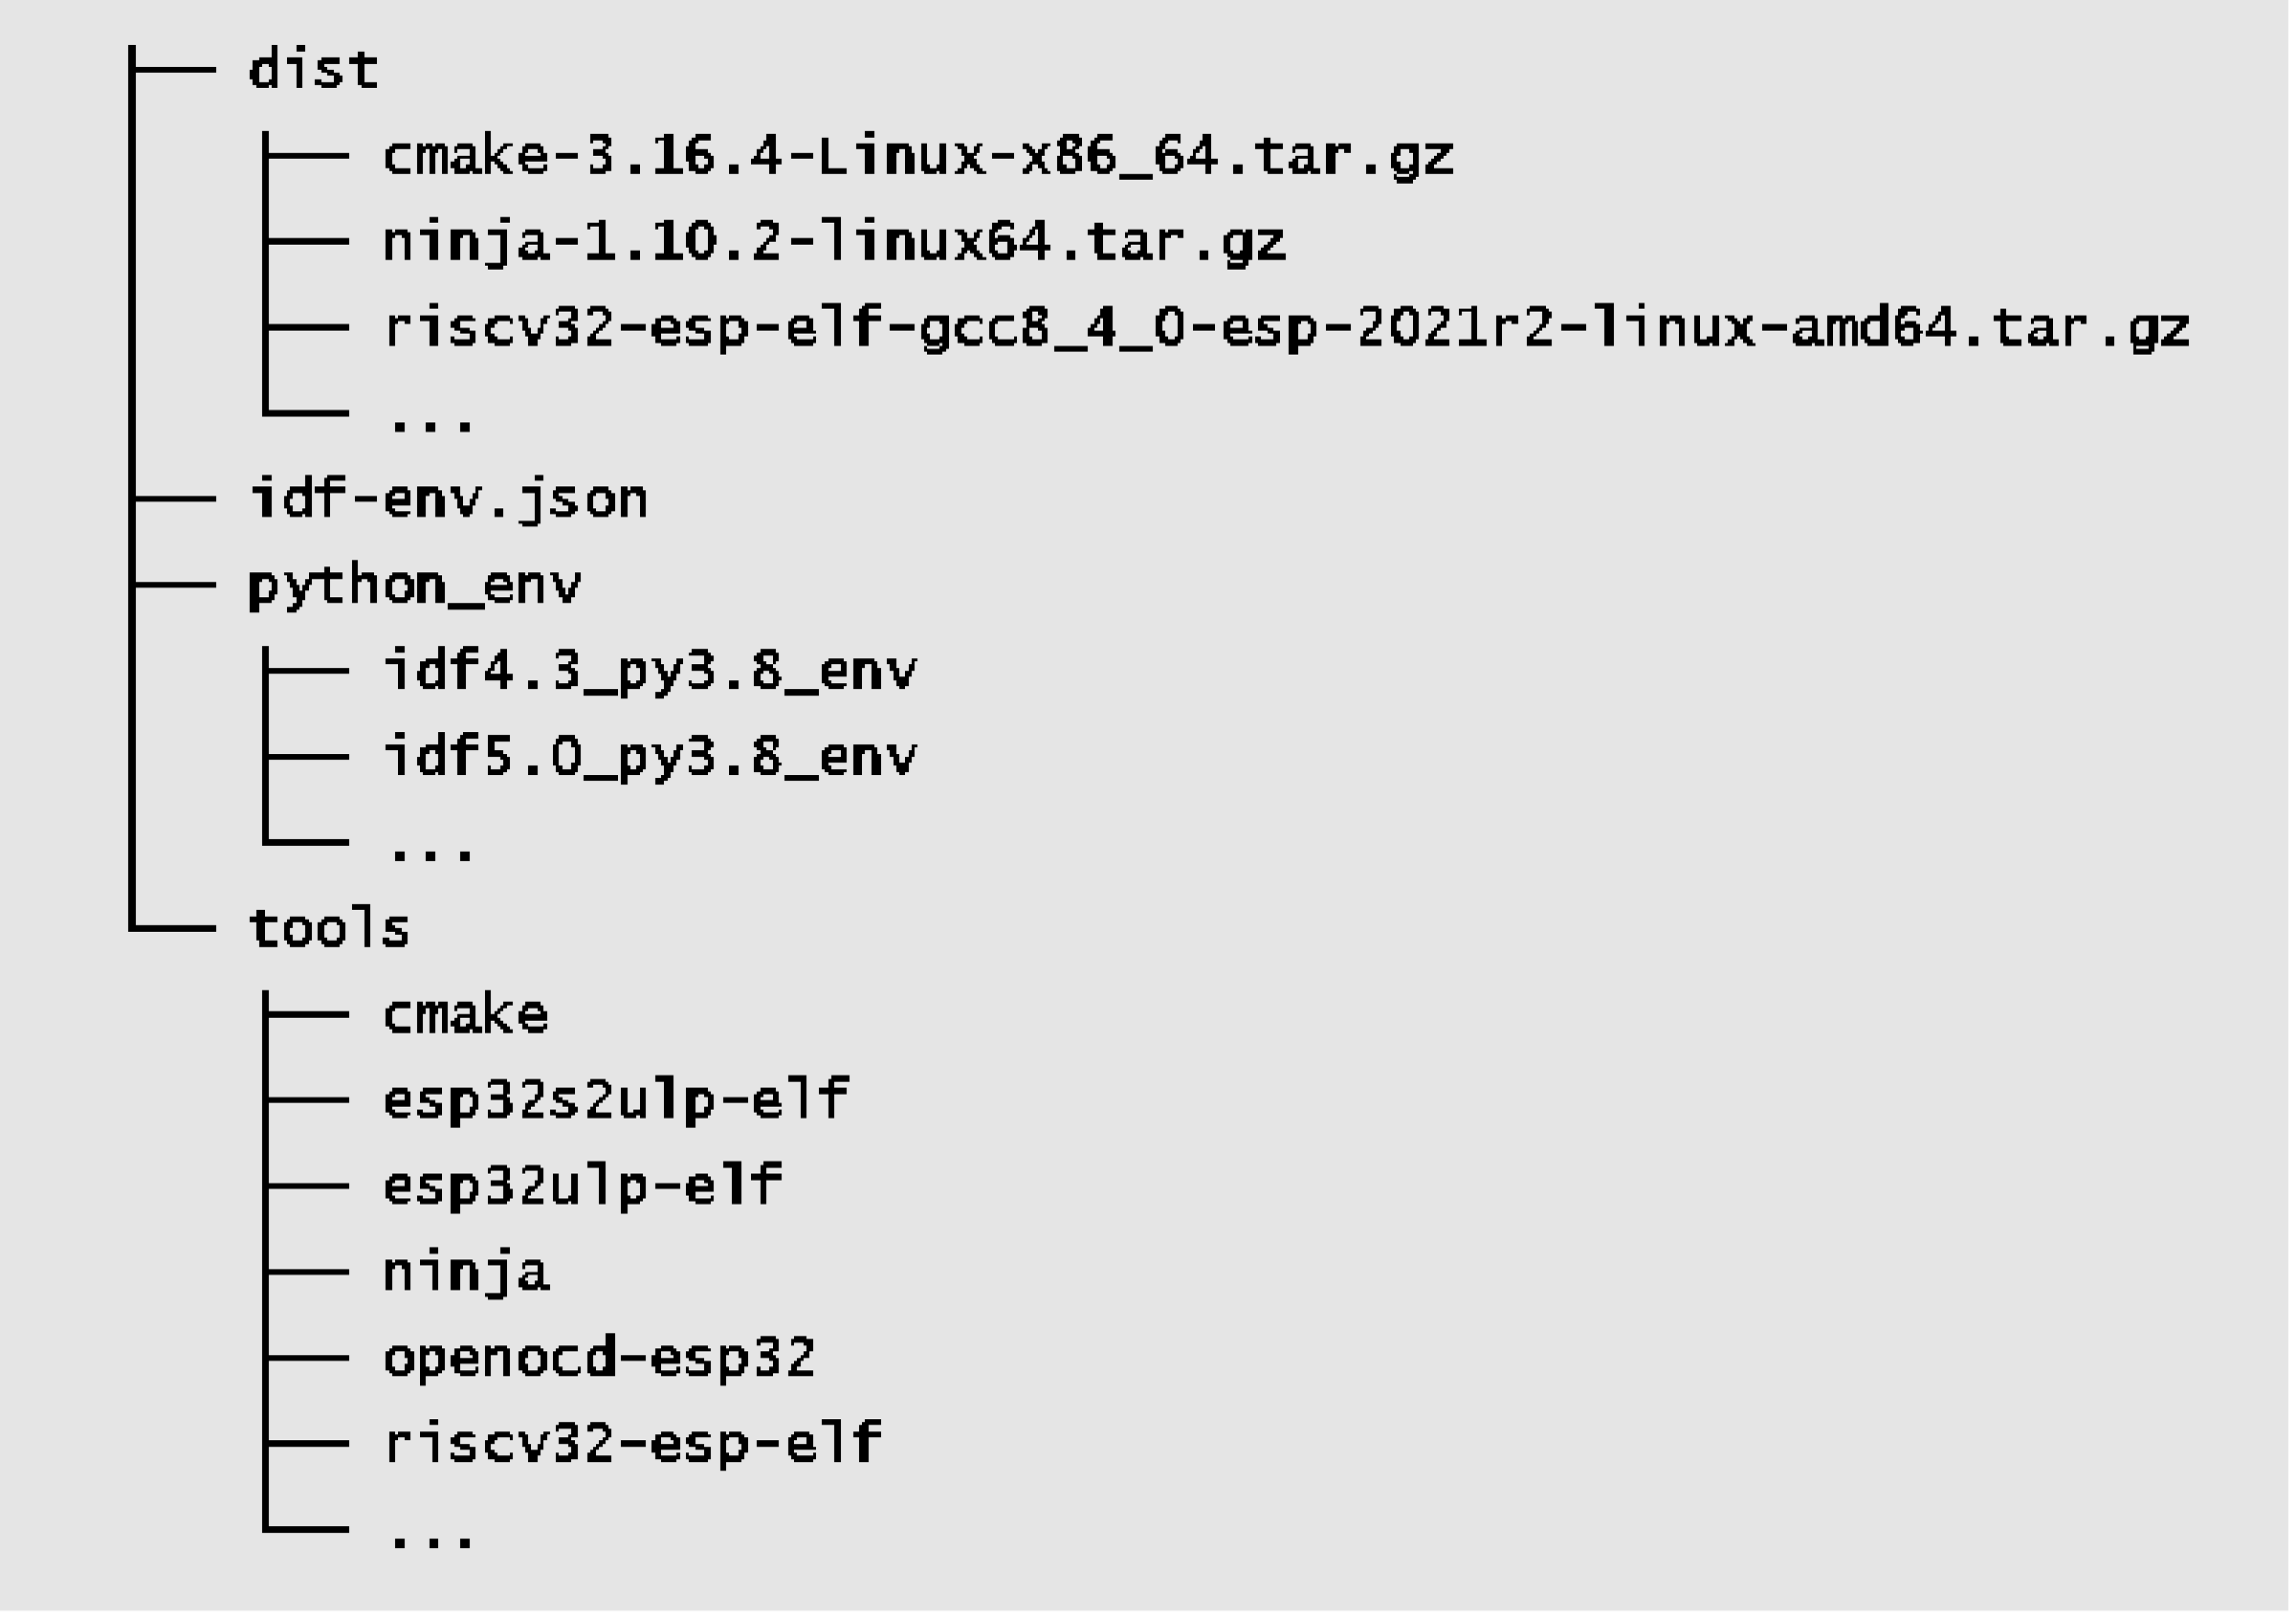
\includegraphics[width=0.75\textwidth]{D4Z/4-3}
        \caption{ESP-IDF compilation tool chain directory}
        \label{ESP-IDF compilation tool chain directory}
    \end{figure}

    \begin{enumerate}[label=\textbf{\alph*.},leftmargin=0em]
        \item \textbf{Software distribution directory \texttt{dist}}

        The ESP-IDF tool chain and other software are distributed in the form of compressed packages. During the installation process, the installation tool first downloads the compressed package to the \verb|dist| directory, and then extracts it to the specified directory. Once the installation is complete, the contents in this directory can be safely removed.

        \item \textbf{Python virtual environment directory \texttt{python\_env}}

        Different versions of ESP-IDF rely on specific versions of Python packages. Installing these packages directly on the same host can lead to conflicts between package versions. To address this, ESP-IDF utilises Python virtual environments to isolate different package versions. With this mechanism, developers can install multiple versions of ESP-IDF on the same host and easily switch between them by importing different environment variables.

        \item \textbf{ESP-IDF compilation tool chain directory \texttt{tools}}

        This directory mainly contains cross-compilation tools required to compile ESP-IDF projects, such as CMake tools, Ninja build tools, and the gcc tool chain that generates the final executable program. Additionally, this directory houses the standard library of the C/C++ language along with the corresponding header files. If a program references a system header file like \verb|#include <stdio.h>|, the compilation tool chain will locate the \verb|stdio.h| file within this directory.
    \end{enumerate}
\end{enumerate}

\section{Setting Up ESP-IDF Development Environment}
The ESP-IDF development environment supports mainstream operating systems such as Windows, Linux, and macOS. This section will introduce how to set up the development environment on each system. It is recommended to develop ESP32-C3 on Linux system, which will be introduced in detail here. Many instructions are applicable across platforms due to the similarity of the development tools. Therefore, it is advised to carefully read the content of this section.

\note{You can refer to the online documents available at
\url{https://bookc3.espressif.com/esp32c3}, which provide the commands mentioned in this section.}

\subsection{Setting up ESP-IDF Development Environment on Linux}
The GNU development and debugging tools required for the ESP-IDF development environment are native to the Linux system. Additionally, the command-line terminal in Linux is powerful and user-friendly, making it an ideal choice for ESP32-C3 development. You can select your preferred Linux distribution, but we recommend using Ubuntu or other Debian-based systems. This section provides guidance on setting up the ESP-IDF development environment on Ubuntu 20.04.

\subsubsection{1. Install required packages}
Open a new terminal and execute the following command to install all necessary packages. The command will automatically skip packages that are already installed.

\begin{codebloc}
\begin{tabular}{d}
\$ \textbf{sudo apt-get install git wget flex bison gperf python3 python3-pip python3- setuptools cmake ninja-build ccache libffi-dev libssl-dev dfu-util libusb-1.0-0}
\end{tabular}
\end{codebloc}

\note[TIPS]{You need to use the administrator account and password for the command above. By default, no information will be displayed when entering the password. Simply press the “Enter” key to continue the procedure.}

Git is a key code management tool in ESP-IDF. After successfully setting up the development environment, you can use the \verb|git log| command to view all code changes made since the creation of ESP-IDF. In addition, Git is also used in ESP-IDF to confirm version information, which is necessary for installing the correct tool chain corresponding to specific versions. Along with Git, other important system tools include Python. ESP-IDF incorporates numerous automation scripts written in Python. Tools such as CMake, Ninja-build, and Ccache are widely used in C/C++ projects and serve as the default code compilation and building tools in ESP-IDF. \verb|libusb-1.0-0| and \verb|dfu-util| are the main drivers used for USB serial communication and firmware burning.

Once the software packages are installed, you can use the \verb|apt show <package_name>| command to obtain detailed descriptions of each package. For example, use \verb|apt show git| to print the description information for the Git tool.

\note[Q: What to do if the Python version is not supported?]{\vspace{3pt}\leftskip 0em \textbf{A:} ESP-IDF v4.3 requires a Python version that is not lower than v3.6. For older versions of Ubuntu, please manually download and install a higher version of Python and set Python3 as the default Python environment. You can find detailed instructions by searching for the keyword \texttt{update-alternatives python}.}

\subsubsection{2. Download ESP-IDF repository code}
Open a terminal and create a folder named \verb|esp| in your home directory using the \verb|mkdir| command. You can choose a different name for the folder if you prefer. Use the \verb|cd| command to enter the folder.

\begin{codebloc}
\begin{tabular}{d}
\$ \textbf{mkdir -p $\sim$/esp}

\$ \textbf{cd $\sim$/esp}
\end{tabular}
\end{codebloc}

Use the \verb|git clone| command to download the ESP-IDF repository code, as shown below:

\begin{codebloc}
\begin{tabular}{d}
\$ \textbf{git clone -b v4.3.2 --recursive https://github.com/espressif/esp-idf.git}
\end{tabular}
\end{codebloc}

In the command above, the parameter \verb|-b v4.3.2| specifies the version to download (in this case, version 4.3.2). The parameter \verb|--recursive| ensures that all sub-repositories of ESP-IDF are downloaded recursively. Information about sub-repositories can be found in the \verb|.gitmodules| file.

\subsubsection{3. Install the ESP-IDF development tool chain}
Espressif provides an automated script \verb|install.sh| to download and install the tool chain. This script checks the current ESP-IDF version and operating system environment, and then downloads and installs appropriate version of Python tool packages and compilation tool chains. The default installation path for the tool chain is \texttt{$\sim$/.espressif}. All you need to do is to navigate to the \verb|esp-idf| directory and run \verb|install.sh|.

\begin{codebloc}
\begin{tabular}{d}
\$ \textbf{cd $\sim$/esp/esp-idf}

\$ \textbf{./install.sh}
\end{tabular}
\end{codebloc}

If you install the the tool chain successfully, the terminal will display:

\begin{codebloc}
\begin{tabular}{d}
All done!
\end{tabular}
\end{codebloc}

At this point, you have successfully set up the ESP-IDF development environment.

\subsection{Setting up ESP-IDF Development Environment on Windows}
\textbf{1. Download ESP-IDF tools installer}

\note[TIPS]{It is recommended to set up the ESP-IDF development environment on Windows 10 or above. You can download the installer from \url{https://dl.espressif.com/dl/esp-idf/}. The installer is also an open-source software, and its source code can be viewed at \url{https://github.com/espressif/idf-installer}.}

\begin{itemize}
    \item \textbf{Online ESP-IDF tools installer}
    
    This installer is relatively small, around 4 MB in size, and other packages and code will be downloaded during the installation process. The advantage of the online installer is that not only can software packages and code be downloaded on demand during the installation process, but also allows the installation of all available releases of ESP-IDF and the latest branch of GitHub code (such as the \verb|master| branch). The disadvantage is that it requires a network connection during the installation process, which may cause installation failure due to network problems.
    
    \item \textbf{Offline ESP-IDF tools installer}
    
    This installer is larger, about 1 GB in size, and contains all the software packages and code required for environment set up. The main advantage of the offline installer is that it can be used on computers without Internet access, and generally has a higher installation success rate. It should be noted that the offline installer can only install stable releases of ESP-IDF identified by v*.* or v*.*.*.
\end{itemize}

\textbf{2. Run the ESP-IDF tools installer}

After downloading a suitable version of the installer (take ESP-IDF Tools Offline 4.3.2 for example here), double-click the exe file to launch the ESP-IDF installation interface. The following demonstrates how to install ESP-IDF stable version v4.3.2 using the offline installer.

\begin{enumerate}[label=(\arabic*)]
    \item In the “Select installation language” interface shown in Figure \ref{“Select installation language” interface}, select the language to be used from the drop-down list.

    \begin{figure}[h!]
        \centering
        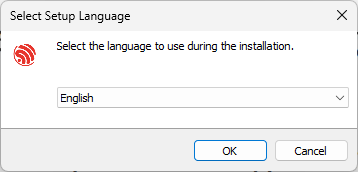
\includegraphics[width=0.41\textwidth]{D4Z/4-4}
        \caption{“Select installation language” interface}
        \label{“Select installation language” interface}
    \end{figure}

    \item After selecting the language, click “OK” to pop up the “License agreement” interface (see Figure \ref{“License agreement” interface}). After carefully reading the installation license agreement, select “I accept the agreement” and click “Next”.

    \begin{figure}[h!]
        \centering
        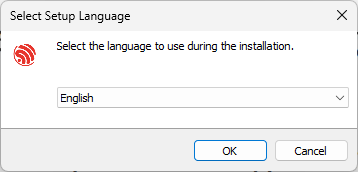
\includegraphics[width=0.53\textwidth]{D4Z/4-5}
        \caption{“License agreement” interface}
        \label{“License agreement” interface}
    \end{figure}

    \item Review the system configuration in the “Pre-installation system check” interface (see Figure \ref{“System check before installation” interface}). Check the Windows version and the installed antivirus software information. Click “Next” if all the configuration items are normal. Otherwise, you can click “Full log” for solutions based on key items.

    \begin{figure}[h!]
        \centering
        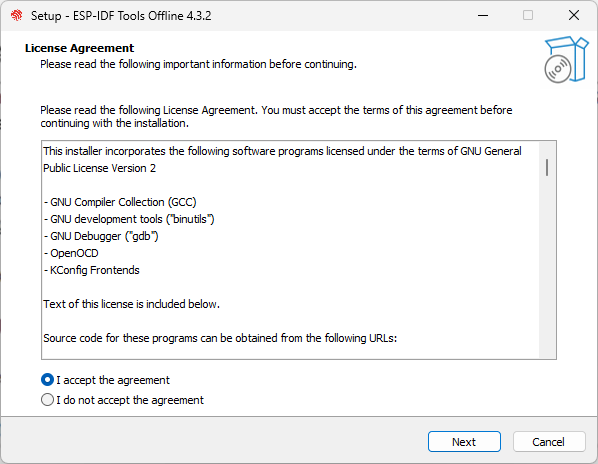
\includegraphics[width=0.53\textwidth]{D4Z/4-6}
        \caption{“System check before installation” interface}
        \label{“System check before installation” interface}
    \end{figure}

    \secnote[TIPS]{You can submit logs to \url{https://github.com/espressif/idf-installer/issues} for help.}

    \item Select the ESP-IDF installation directory. Here, select \verb|D:/.espressif|, as shown in Figure \ref{Select the ESP-IDF installation directory}, and click “Next”. Please note that \verb|.espressif| here is a hidden directory. After the installation is completed, you can view the specific contents of this directory by opening the file manager and displaying hidden items.

    \begin{figure}[h!]
        \centering
        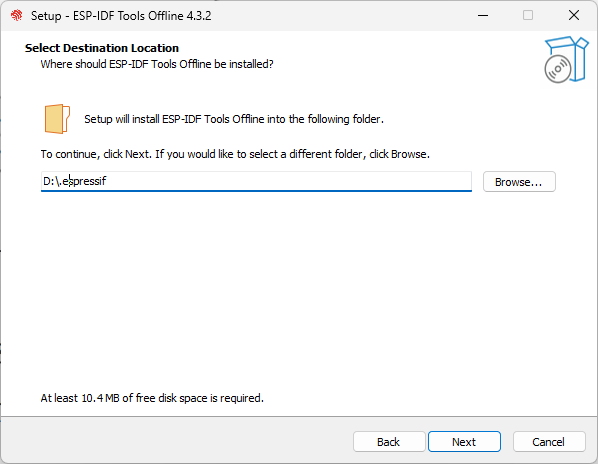
\includegraphics[width=0.53\textwidth]{D4Z/4-7}
        \caption{Select the ESP-IDF installation directory}
        \label{Select the ESP-IDF installation directory}
    \end{figure}

    \item Check the components that need to be installed, as shown in Figure \ref{Select the components to install}. It is recommended to use the default option, that is, complete installation, and then click “Next”.

    \begin{figure}[h!]
        \centering
        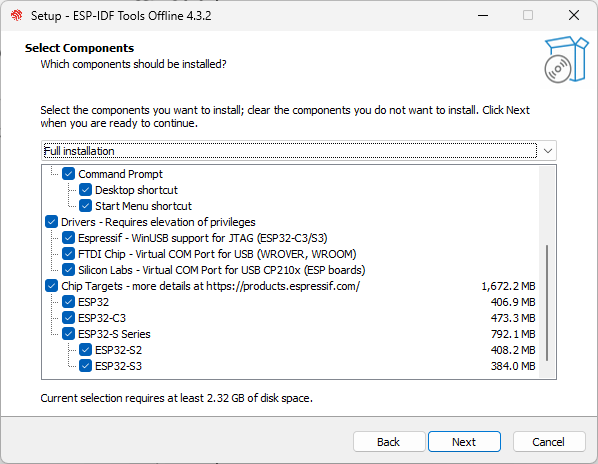
\includegraphics[width=0.55\textwidth]{D4Z/4-8}
        \caption{Select the components to install}
        \label{Select the components to install}
    \end{figure}

    \item Confirm the components to be installed and click “Install” to start the automated installation process, as shown in Figure \ref{Preparing for installation}. The installation process may last tens of minutes and the progress bar of the installation process is shown in Figure \ref{Installation progress bar}. Please wait patiently.

    \begin{figure}[h!]
        \centering
        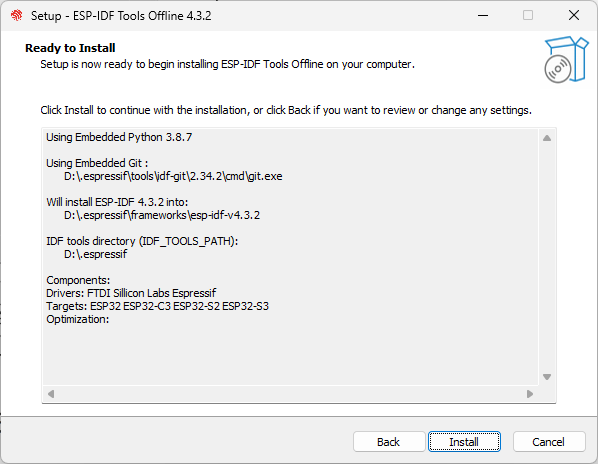
\includegraphics[width=0.55\textwidth]{D4Z/4-9}
        \caption{Preparing for installation}
        \label{Preparing for installation}
    \end{figure}

    \begin{figure}[h!]
        \centering
        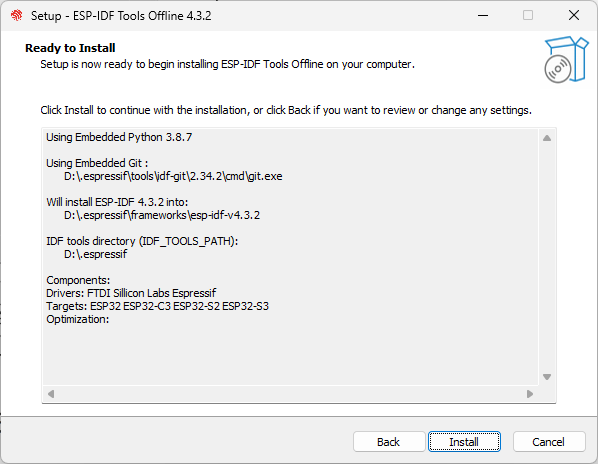
\includegraphics[width=0.55\textwidth]{D4Z/4-10}
        \caption{Installation progress bar}
        \label{Installation progress bar}
    \end{figure}

    \item After the installation is complete, it is recommended to check “Register the ESP-IDF Tools executables as Windows Defender exclusions...” to prevent antivirus software from deleting files. Adding exclusion items can also skip frequent scans by antivirus software, greatly improving the code compilation efficiency of the Windows system. Click “Finish” to complete the installation of the development environment, as shown in Figure \ref{Installation completed}. You can choose to check “Run ESP-IDF PowerShell environment” or “Run ESP-IDF command prompt”. Run the compilation window directly after installation to ensure that the development environment functions normally.

    \begin{figure}[h!]
        \centering
        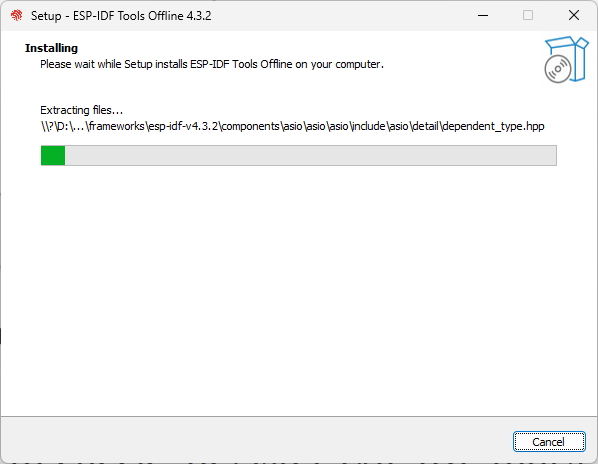
\includegraphics[width=0.55\textwidth]{D4Z/4-11}
        \caption{Installation completed}
        \label{Installation completed}
    \end{figure}

    \item Open the installed development environment in the program list (either ESP-IDF 4.3 CMD or ESP-IDF 4.3 PowerShell terminal, as shown in Figure \ref{Development environment installed}), and the ESP-IDF environment variable will be automatically added when running in the terminal. After that, you can use the \verb|idf.py| command for operations. The opened ESP-IDF 4.3 CMD is shown in Figure \ref{ESP-IDF 4.3 CMD}.

    \begin{figure}[h!]
        \centering
        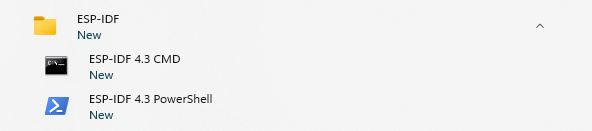
\includegraphics[width=0.4\textwidth,frame]{D4Z/4-12}
        \caption{Development environment installed}
        \label{Development environment installed}
    \end{figure}

    \begin{figure}[h!]
        \centering
        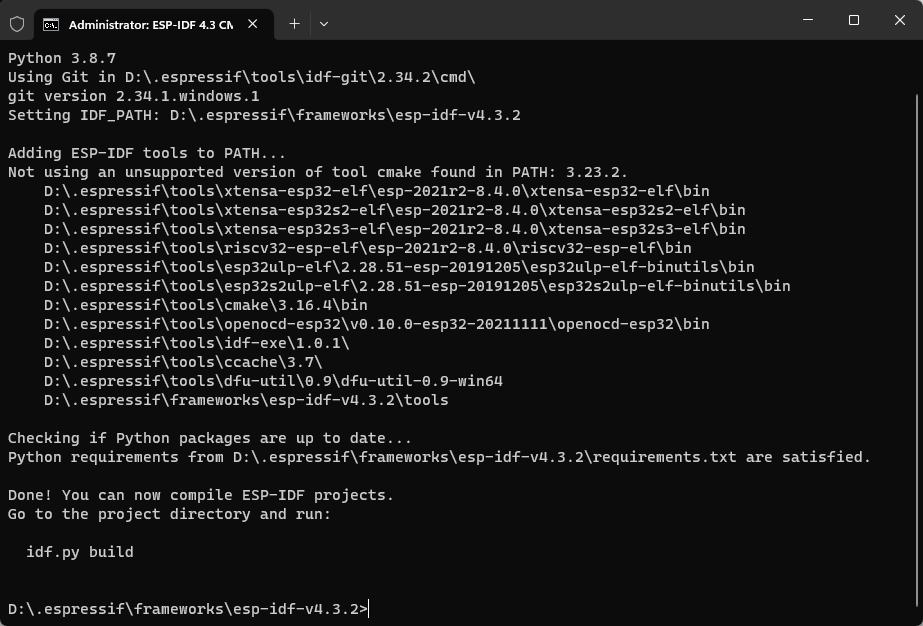
\includegraphics[width=0.55\textwidth]{D4Z/4-13}
        \caption{ESP-IDF 4.3 CMD}
        \label{ESP-IDF 4.3 CMD}
    \end{figure}
\end{enumerate}

\subsection{Setting up ESP-IDF Development Environment on Mac}
The process of installing the ESP-IDF development environment on a Mac system is the same as that on a Linux system. The commands for downloading the repository code and installing the tool chain are exactly the same. Only the commands for installing dependency packages are slightly different.

\textbf{1. Install dependency packages}

Open a terminal, and install pip, the Python package management tool, by running the following command:

\begin{codebloc}
\begin{tabular}{d}
\% \textbf{sudo easy\_install pip}
\end{tabular}
\end{codebloc}

Install Homebrew, a package management tool for macOS, by running the following command:

\begin{codebloc}
\begin{tabular}{d}
\% \textbf{/bin/bash -c "\$(curl -fsSL https://raw.githubusercontent.com/Homebrew/install/\newline HEAD/install.sh)"}
\end{tabular}
\end{codebloc}

Install the required dependency packages by running the following command:

\begin{codebloc}
\begin{tabular}{d}
\% \textbf{brew python3 install cmake ninja ccache dfu-util}
\end{tabular}
\end{codebloc}

\textbf{2. Download ESP-IDF repository code}

Follow the instructions provided in section 4.2.1 to download the ESP-IDF repository code. The steps are the same as for downloading on a Linux system.

\textbf{3. Install the ESP-IDF development tool chain}

Follow the instructions provided in section 4.2.1 to install the ESP-IDF development tool chain. The steps are the same as for installation on a Linux system.

\subsection{Installing VS Code}
By default, the ESP-IDF SDK does not include a code editing tool (though the latest ESP-IDF installer for Windows offers the option to install ESP-IDF Eclipse). You can use any text editing tool of your choice to edit the code and then compile it using terminal commands.

One popular code editing tool is VS Code (Visual Studio Code), which is a free and feature-rich code editor with a user-friendly interface. It offers various plugins that provide functionalities such as code navigation, syntax highlighting, Git version control, and terminal integration. Additionally, Espressif has developed a dedicated plugin called Espressif IDF for VS Code, which simplifies project configuration and debugging.

You can use the \verb|code| command in the terminal to quickly open the current folder in VS Code. Alternatively, you can use the shortcut \texttt{Ctrl+$\sim$} to open the system’s default terminal console within VS Code.

\note[TIPS]{It is recommended to use VS Code for ESP32-C3 code development. Download and install the latest version of VS Code at \url{https://code.visualstudio.com/}.}

\subsection{Introduction to Third-Party Development Environments}
In addition to the official ESP-IDF development environment, which primarily uses the C language, ESP32-C3 also supports other mainstream programming languages and a wide range of third-party development environments. Some notable options include:

\begin{term}{Arduino:}
    an open-source platform for both hardware and software, supporting various microcontrollers, including ESP32-C3.
    
    \vspace{6pt}
    It uses the C++ language and offers a simplified and standardised API, commonly referred to as the Arduino language. Arduino is widely used in prototype development and educational contexts. It provides an extensible software package and an IDE that allows for easy compilation and flashing.
\end{term}

\begin{term}{MicroPython:}
    a Python 3 language interpreter designed to run on embedded microcontroller platforms.
    
    \vspace{6pt}
    With a simple script language, it can directly access ESP32-C3’s peripheral resources (such as UART, SPI, and I2C) and communication functions (such as Wi-Fi and Bluetooth LE). This simplifies hardware interaction. MicroPython, combined with Python’s extensive mathematical operation library, enables the implementation of complex algorithms on ESP32-C3, facilitating the development of AI-related applications. As a script language, there is no need for repeated compilation; modifications can be made and scripts can be executed directly.
\end{term}

\begin{term}{NodeMCU:}
    an LUA language interpreter developed for ESP series chips.
    
    \vspace{6pt}
    It supports almost all peripheral functions of ESP chips and is lighter than MicroPython. Similar to MicroPython, NodeMCU uses a script language, eliminating the need for repeated compilation.
\end{term}

Furthermore, ESP32-C3 also supports the NuttX and Zephyr operating systems. NuttX is a real-time operating system that provides POSIX-compatible interfaces, enhancing application portability. Zephyr is a small real-time operating system specifically designed for IoT applications. It includes numerous software libraries required in IoT development, gradually evolving into a comprehensive software ecosystem.

This book does not provide detailed installation instructions for the aforementioned development environments. You can install a development environment based on your requirements by following the respective documentation and instructions.

\section{ESP-IDF Compilation System}
\subsection{Basic Concepts of Compilation System}
An ESP-IDF project is a collection of a main program with an entry function and multiple independent functional components. For example, a project that controls LED switches mainly consists of an entry program \verb|main| and a \verb|driver| component that controls GPIO. If you want to realise the LED remote control, you also need to add Wi-Fi, TCP/IP protocol stack, etc.

The compilation system can compile, link, and generate executable files (.bin) for the code through a set of building rules. The compilation system of ESP-IDF v4.0 and above versions is based on CMake by default, and the compilation script \verb|CMakeLists.txt| can be used to control the compilation behavior of the code. In addition to supporting the basic syntax of CMake, the ESP-IDF compilation system also defines a set of default compilation rules and CMake functions, and you can write the compilation script with simple statements.

\subsection{Project File Structure}
A project is a folder that contains an entry program \verb|main|, user-defined components, and files required to build executable applications, such as compilation scripts, configuration files, partition tables, etc. Projects can be copied and passed on, and the same executable file can be compiled and generated in machines with the same version of ESP-IDF development environment. A typical ESP-IDF project file structure is shown in Figure \ref{Typical ESP-IDF project file structure}.

\begin{figure}[h!]
    \centering
    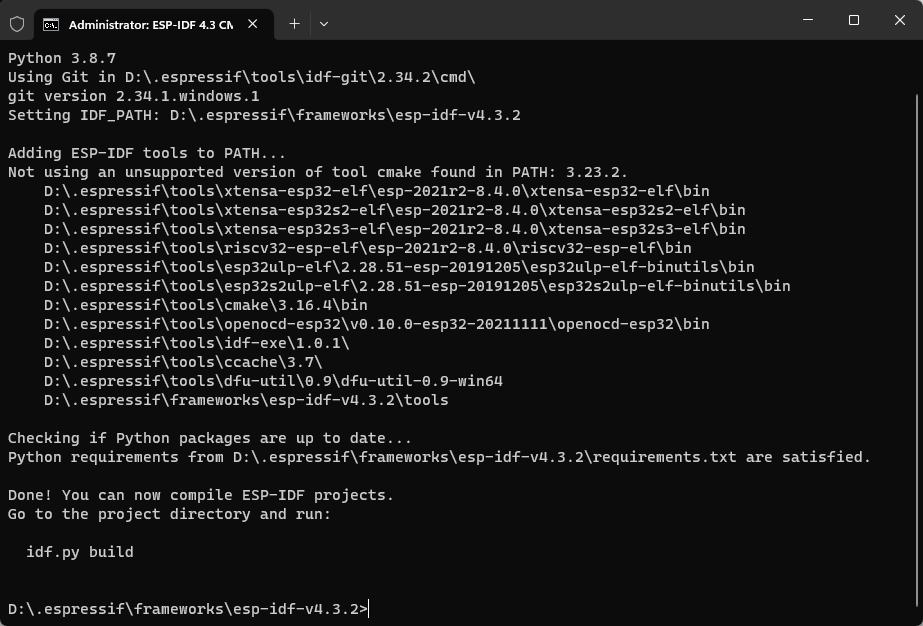
\includegraphics[width=0.35\textwidth]{D4Z/4-14}
    \caption{Typical ESP-IDF project file structure}
    \label{Typical ESP-IDF project file structure}
\end{figure}

Since ESP-IDF supports multiple IoT chips from Espressif, including ESP32, ESP32-S series, ESP32-C series, ESP32-H series, etc., a target needs to be determined before compiling the code. The target is both the hardware device that runs the application program and the build target of the compilation system.

Depending on your needs, you can specify one or more targets for your project. For example, through command \verb|idf.py set-target esp32c3|, you can set the compilation target to ESP32-C3, during which the default parameters and compilation tool chain path for ESP32-C3 will be loaded. After compilation, an executable program can be generated for ESP32-C3. You can also run the command \verb|set-target| again to set a different target, and the compilation system will automatically clean up and reconfigure.

\begin{term}{Components}
    Components in ESP-IDF are modular and independent code units managed within the compilation system. They are organised as folders, with the folder name representing the component name by default. Each component has its own compilation script that specifies its compilation parameters and dependencies. During the compilation process, components are compiled into separate static libraries (.a files) and eventually combined with other components to form the application program.

    \parskip 6pt
    ESP-IDF provides essential functions, such as the operating system, peripheral drivers, and network protocol stack, in the form of components. These components are stored in the \verb|components| directory located within the ESP-IDF root directory. Developers do not need to copy these components to the \verb|components| directory of \verb|myProject|. Instead, they only need to specify the dependency relationships of these components in the project’s \verb|CMakeLists.txt| file using the \verb|REQUIRES| or \verb|PRIV_REQUIRES| directives. The compilation system will automatically locate and compile the required components.

    Therefore, the \verb|components| directory under \verb|myProject| is not necessary. It is only used to include some custom components of the project, which can be third-party libraries or user-defined code. Additionally, components can be sourced from any directory other than ESP-IDF or the current project, such as from an open-source project saved in another directory. In this case, you only need to add the path of the component by setting the \verb|EXTRA_COMPONENT_DIRS| variable in the \verb|CMakeLists.txt| under the root directory. This directory will override any ESP-IDF component with the same name, ensuring the correct component is used.
\end{term}

\begin{term}{Entry program \texttt{main}}
    The \verb|main| directory within the project follows the same file structure as other components (e.g., \verb|component1|). However, it holds a special significance as it is a mandatory component that must exist in every project. The main directory contains the project’s source code and the user program’s entry point, typically named \verb|app_main|. By default, the execution of the user program starts from this entry point. The \verb|main| component also differs in that it automatically depends on all components within the search path. Therefore, there is no need to explicitly indicate dependencies using the \verb|REQUIRES| or \verb|PRIV_REQUIRES| directives in the \verb|CMakeLists.txt| file.
\end{term}

\begin{term}{Configuration file}
    The root directory of the project contains a configuration file called \verb|sdkconfig|, which contains the configuration parameters for all the components within the project. The \verb|sdkconfig| file is automatically generated by the compilation system and can be modified and regenerated by the command \verb|idf.py menuconfig|. The menuconfig options mainly originate from the \verb|Kconfig.projbuild| of the project and the \verb|Kconfig| of the components. Component developers generally add configuration items in \verb|Kconfig| to make the component flexible and configurable.
\end{term}

\begin{term}{\texttt{Build} directory}
    By default, the \verb|build| directory within the project stores intermediate files and the final executable programs generated by the \verb|idf.py build| command. In general, it is not necessary to directly access the contents of the \verb|build| directory. ESP-IDF provides predefined commands to interact with the directory, such as using the \verb|idf.py flash| command to automatically locate the compiled binary file and flash it to the specified flash address, or using the \verb|idf.py fullclean| command to clean the entire \verb|build| directory.
\end{term}

\begin{term}{Partition table (\texttt{partitions.csv})}
    Each project requires a partition table to divide the space of flash and specify the size and starting address of the executable program and user data space. Command \verb|idf.py |\\ \verb|flash| or OTA upgrade program will flash the firmware to the corresponding address according to this table. ESP-IDF provides several default partition tables in \verb|components/|\\ \verb|partition_table|, such as \verb|partitions_singleapp.csv| and \verb|partitions_two_|\\ \verb|ota.csv|, which can be selected in \verb|menuconfig|.
    
    \vspace{6pt}
    If the default partition table of the system cannot meet the requirements of the project, a custom \verb|partitions.csv| can be added to the project directory and be selected in \verb|menuconfig|.
\end{term}

\subsection{Default Build Rules of the Compilation System}
\begin{term}{Rules for overriding components with the same name}
    During the component search process, the compilation system follows a specific order. It first searches for internal components of ESP-IDF, then looks for components of the user project, and finally searches for components in \verb|EXTRA_COMPONENT_DIRS|. In cases where multiple directories contain components with the same name, the component found in the last directory will override any previous components with the same name. This rule allows for the customisation of ESP-IDF components within the user project, while keeping the original ESP-IDF code intact.
\end{term}

\begin{term}{Rules for including common components by default}
    As mentioned in section 4.3.2, components need to explicitly specify their dependencies on other components in the \verb|CMakeLists.txt|. However, common components such as \verb|freertos| are automatically included in the build system by default, even if their dependency relationships are not explicitly defined in the compilation script. ESP-IDF common components include \verb|freertos|, \verb|Newlib|, \verb|heap|, \verb|log|, \verb|soc|, \verb|esp_rom|, \verb|esp_common|, \verb|xtensa/riscv|, and \verb|cxx|. Using these common components avoids repetitive work when writing \verb|CMakeLists.txt| and make it more concise.
\end{term}

\begin{term}{Rules for overriding configuration items}
    Developers can add default configuration parameters by adding a default configuration file named \verb|sdkconfig.defaults| to the project. For example, adding \verb|CONFIG_LOG_|\\ \verb|DEFAULT_LEVEL_NONE = y| can configure the UART interface to not print log data by default. Furthermore, if specific parameters need to be set for a particular target, a configuration file named \verb|sdkconfig.defaults.TARGET_NAME| can be added, where \verb|TARGET_NAME| can be \verb|esp32s2|, \verb|esp32c3|, and so on. These configuration files are imported into the \verb|sdkconfig| during compilation, with the general default configuration file \verb|sdkconfig.defaults| being imported first, followed by the target-specific configuration file, such as \verb|sdkconfig.defaults.esp32c3|. In cases where there are configuration items with the same name, the latter configuration file will override the former.
\end{term}

\subsection{Introduction to the Compilation Script}
When developing a project using ESP-IDF, developers not only need to write source code but also need to write \verb|CMakeLists.txt| for the project and components. \verb|CMakeLists.txt| is a text file, also known as a compilation script, which defines a series of compilation objects, compilation configuration items, and commands to guide the compilation process of the source code. The compilation system of ESP-IDF v4.3.2 is based on CMake. In addition to supporting native CMake functions and commands, it also defines a series of custom functions, making it much easier to write compilation scripts.

The compilation scripts in ESP-IDF mainly include the project compilation script and the component compilation scripts. The \verb|CMakeLists.txt| in the root directory of the project is called the project compilation script, which guides the compilation process of the entire project. A basic project compilation script typically includes the following three lines:

\begin{codebloc}
\begin{tabular}{d}
\verb|1.  cmake_minimum_required(VERSION 3.5)|

\verb|2.  include($ENV{IDF_PATH}/tools/cmake/project.cmake)|

\verb|3.  project(myProject)|
\end{tabular}
\end{codebloc}

Among them, the \verb|cmake_minimum_required (VERSION 3.5)| must be placed on the first line, which is used to indicate the minimum CMake version number required by the project. Newer versions of CMake are generally backward compatible with older versions, so adjust the version number accordingly when using newer CMake commands to ensure compatibility.

\verb|include($ENV {IDF_PATH}/tools/cmake/project.cmake)| imports pre-defined\\ configuration items and commands of ESP-IDF compilation system, including the default build rules of the compilation system described in Section 4.3.3. \verb|project(myProject)| creates the project itself and specifies its name. This name will be used as the final output binary file name, i.e., \verb|myProject.elf| and \verb|myProject.bin|.

A project can have multiple components, including the \verb|main| component. The top-level directory of each component contains a \verb|CMakeLists.txt| file, which is called the component compilation script. Component compilation scripts are mainly used to specify component dependencies, configuration parameters, source code files, and included header files for compilation. With ESP-IDF’s custom function \verb|idf_component_register|, the minimum required code for a component compilation script is as follows:

\begin{codebloc}
\begin{tabular}{d}
\verb|1.  idf_component_register(SRCS "src1.c"|

\verb|2.                        INCLUDE_DIRS "include"|

\verb|3.                        REQUIRES component1)|
\end{tabular}
\end{codebloc}

The \verb|SRCS| parameter provides a list of source files in the component, separated by spaces if there are multiple files. The \verb|INCLUDE_DIRS| parameter provides a list of public header file directories for the component, which will be added to the \verb|include| search path for other components that depend on the current component. The \verb|REQUIRES| parameter identifies the public component dependencies for the current component. It is necessary for components to explicitly state which components they depend on, such as \verb|component2| depending on \verb|component1|. However, for the \verb|main| component, which depends on all components by default, the \verb|REQUIRES| parameter can be omitted.

In addition, native CMake commands can also be used in the compilation script. For example, use the command \verb|set| to set variables, such as \verb|set(VARIABLE "VALUE")|.

\subsection{Introduction to Common Commands}
ESP-IDF uses CMake (project configuration tool), Ninja (project building tool) and esptool (flash tool) in the process of code compilation. Each tool plays a different role in the compilation, building, and flash process, and also supports different operating commands. To facilitate user operation, ESP-IDF adds a unified front-end \verb|idf.py| that allows the above commands to be called quickly.

Before using \verb|idf.py|, make sure that:

\begin{itemize}[leftmargin=1.5em, noitemsep]
    \item The environment variable \verb|IDF_PATH| of ESP-IDF has been added to the current terminal.
    \item The command execution directory is the root directory of the project, which includes the project compilation script \verb|CMakeLists.txt|.
\end{itemize}

The common commands of \verb|idf.py| are as follows:

\begin{itemize}[leftmargin=1.5em, noitemsep]
    \item \verb|idf.py --help|: displaying a list of commands and their usage instructions.
    \item \verb|idf.py set-target <target>|: setting the compilation taidf.py fullcleanrget, such as replacing \verb|<target>| with \verb|esp32c3|.
    \item \verb|idf.py menuconfig|: launching \verb|menuconfig|, a terminal graphical configuration tool, which can select or modify configuration options, and the configuration results are saved in the \verb|sdkconfig| file.
    \item \verb|idf.py build|: initiating code compilation. The intermediate files and the final executable program generated by the compilation will be saved in the \verb|build| directory of the project by default. The compilation process is incremental, which means that if only one source file is modified, only the modified file will be compiled next time.
    \item \verb|idf.py clean|: cleaning the intermediate files generated by the project compilation. The entire project will be forced to compile in the next compilation. Note that the CMake configuration and the configuration modifications made by \verb|menuconfig| will not be deleted during cleanup.
    \item \verb|idf.py fullclean|: deleting the entire \verb|build| directory, including all CMake configuration output files. When building the project again, CMake will configure the project from scratch. Please note that this command will recursively delete all files in the build directory, so use it with caution, and the project configuration file will not be deleted.
    \item \verb|idf.py flash|: flashing the executable program binary file generated by \verb|build| to the target ESP32-C3. The options \verb|-p <port_name>| and \verb|-b <baud_rate>| are used to set the device name of the serial port and the baud rate for flashing, respectively. If these two options are not specified, the serial port will be automatically detected and the default baud rate will be used.
    \item \verb|idf.py monitor|: displaying the serial port output of the target ESP32-C3. The option \verb|-p| can be used to specify the device name of the host-side serial port. During serial port printing, press the key combination \verb|Ctrl+]| to exit the monitor.
\end{itemize}

The above commands can also be combined as needed. For example, the command \verb|idf.py |\\ \verb|build flash monitor| will perform code compilation, flash, and open the serial port monitor in sequence.

You can visit \url{https://bookc3.espressif.com/build-system} to know more about ESP-IDF compilation system.

\section{Practice: Compiling Example Program “Blink”}
\subsection{Example Analysis}
This section will take the program Blink as an example to analyse the file structure and coding rules of a real project in detail. The Blink program implements the LED blinking effect, and the project is located in the directory \verb|examples/get-started/blink|, which contains a source file, configuration files, and several compilation scripts.

The smart light project introduced in this book is based on this example program. Functions will be gradually added in later chapters to finally complete it.

\note[Source code]{In order to demonstrate the entire development process, the Blink program has been copied to \href{https://github.com/espressif/book-esp32c3-iot-projects/tree/main/device_firmware/1_blink}{\texttt{esp32c3-iot-projects/device\_firmware/1\_blink}}.}

The directory structure of the \verb|blink| project files is shown in Figure \ref{File directory structure of the blink project}.

\begin{figure}[h!]
    \centering
    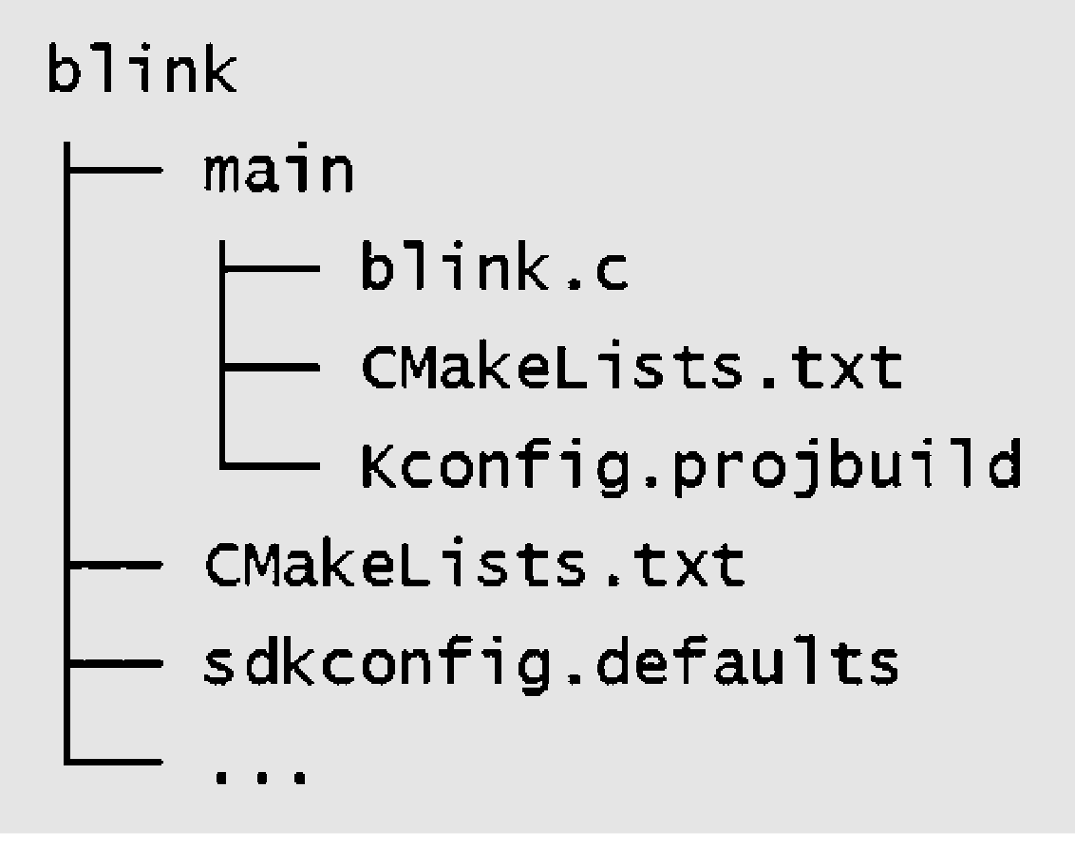
\includegraphics[width=0.3\textwidth]{D4Z/4-15}
    \caption{File directory structure of the \texttt{blink} project}
    \label{File directory structure of the blink project}
\end{figure}

The \verb|blink| project contains only one \verb|main| directory, which is a special component that must be included as described in section 4.3.2. The main directory is mainly used to store the implementation of the \verb|app_main()| function, which is the entry point to the user program.The \verb|blink| project does not include the \verb|components| directory, because this example only needs to use the components that come with ESP-IDF and does not require additional components. The \verb|CMakeLists.txt| included in the \verb|blink| project is used to guide the compilation process, while \verb|Kconfig.projbuild| is used to add configuration items for this example program in \verb|menuconfig|. Other unnecessary files will not affect the compilation of the code, so they will not be discussed here. A detailed introduction to the \verb|blink| project files is as follows.

\begin{codebloc}
\begin{tabular}{d}
\vspace{2pt}
\begin{verbatim}
1.  /*blink.c includes the following header files*/
2.  #include <stdio.h>              //Standard C library header file
3.  #include "freertos/freeRTOS.h"  //FreeRTOS main header file
4.  #include "freertos/task.h"      //FreeRTOS Task header file
5.  #include "sdkconfig.h"      //Configuration header file generated by kconfig
\end{verbatim}
\verb|6.  #include "driver/gpio.h"        //GPIO driver header file|
\end{tabular}
\end{codebloc}

The source file \verb|blink.c| contains a series of header files corresponding to function declarations. ESP-IDF generally follows the order of including standard library header files, FreeRTOS header files, driver header files, other component header files, and project header files. The order in which header files are included may affect the final compilation result, so try to follow the default rules. It should be noted that \verb|sdkconfig.h| is automatically generated by \verb|kconfig| and can only be configured through the command \verb|idf.py menuconfig|. Direct modification of this header file will be overwritten.

\begin{codebloc}
\begin{tabular}{d}
\vspace{2pt}
\begin{verbatim}
1.  /*You can select the GPIO corresponding to the LED in idf.py menuconfig,
    and the modification result of menuconfig is that the value of CONFIG_BLINK
    _GPIO will be changed. You can also directly modify the macro definition 
    here, and change CONFIG_BLINK_GPIO to a fixed value.*/
2.  #define BLINK_GPIO CONFIG_BLINK_GPIO
3.  void app_main(void)
4.  {
5.      /*Configure IO as the GPIO default function, enable pull-up mode, and
6.      disable input and output modes*/
\end{verbatim}
\verb|7.      gpio_reset_pin(BLINK_GPIO);|
\end{tabular}
\end{codebloc}

\begin{codebloc}
\begin{tabular}{d}
\vspace{2pt}
\begin{verbatim}
8.      /*Set GPIO to output mode*/
9.      gpio_set_direction(BLINK_GPIO, GPIO_MODE_OUTPUT);
10.     while(1) {
11.         /*Print log*/
12.         printf("Turning off the LED\n");
13.         /*Turn off the LED (output low level)*/
14.         gpio_set_level(BLINK_GPIO, 0);
15.         /*Delay (1000 ms)*/
16.         vTaskDelay(1000 / portTICK_PERIOD_MS);
17.         printf("Turning on the LED\n");
18.         /*Turn on the LED (output high level)*/
19.         gpio_set_level(BLINK_GPIO, 1);
20.         vTaskDelay(1000 / portTICK_PERIOD_MS);
21.     }
\end{verbatim}
\verb|22. }|
\end{tabular}
\end{codebloc}

The \verb|app_main()| function in the Blink example program serves as the entry point for user programs. It is a simple function with no parameters and no return value. This function is called after the system has completed initialisation, which includes tasks such as initialising the log serial port, configuring single/dual core, and configuring the watchdog.

The \verb|app_main()| function runs in the context of a task named \verb|main|. The stack size and priority of this task can be adjusted in \verb|menuconfig → Componentconfig → Common |\\ \verb|ESP-related|.

For simple tasks like blinking an LED, all the necessary code can be implemented directly in the \verb|app_main()| function. This typically involves initialising the GPIO corresponding to the LED and using a \verb|while(1)| loop to toggle the LED on and off. Alternatively, you can use FreeRTOS API to create a new task that handles the LED blinking. Once the new task is successfully created, you can exit the \verb|app_main()| function.

The content of \verb|main/CMakeLists.txt| file, which guides the compilation process for the main component, is as follows:

\begin{codebloc}
\begin{tabular}{d}
\verb|1.  idf_component_register(SRCS "blink.c" INCLUDE_DIRS "." )|
\end{tabular}
\end{codebloc}

Among them, \verb|main/CMakeLists.txt| only calls one compilation system function, that is \verb|idf_component_register|. Similar to the \verb|CMakeLists.txt| for most other components, \verb|blink.c| is added to \verb|SRCS|, and the source files added to \verb|SRCS| will be compiled. At the same time, “\verb|.|”, which represents the path where \verb|CMakeLists.txt| is located, should be added to \verb|INCLUDE_DIRS| as the search directories for header files. The content of \verb|CMakeLists.txt| is as follows:

\begin{codebloc}
\begin{tabular}{d}
\vspace{2pt}
\begin{verbatim}
1.  #Specify v3.5 as the oldest CMake version supported by the current project
2.  #Versions lower than v3.5 must be upgraded before compilation continues
3.  cmake_minimum_required(VERSION 3.5)
\end{verbatim}
\verb|4.  #Include the default CMake configuration of the ESP-IDF compilation system|
\end{tabular}
\end{codebloc}

\begin{codebloc}
\begin{tabular}{d}
\vspace{2pt}
\begin{verbatim}
5.  include($ENV{IDF_PATH}/tools/cmake/project.cmake)
6.  #Create a project named "blink"
\end{verbatim}
\verb|7.  project(myProject)|
\end{tabular}
\end{codebloc}

Among them, the \verb|CMakeLists.txt| in the root directory mainly includes \verb|$ENV{IDF_|\\ \verb|PATH}/tools/cmake/project.cmake|, which is the main CMake configuration file provided by ESP-IDF. It is used to configure the default rules of the ESP-IDF compilation system and define common functions such as \verb|idf_component_register|; \verb|project(blink)| creates a project called \verb|blink|, and the final firmware will be named \verb|blink.bin|.

\subsection{Compiling the Blink Program}
This section takes the Blink program as an example to demonstrate the compilation process of a simple ESP-IDF program. It is important to note that this section uses the high/low level of GPIO to drive the LED. However, the WS2812 indicator light requires a special communication protocol. You can refer to the example program in \href{https://github.com/espressif/esp-idf/tree/master/examples/peripherals/rmt/led_strip}{\texttt{esp-idf/examples/periphe-\\ rals/rmt/led\_strip}} for more information.

\subsubsection{1. Open a new terminal and import the ESP-IDF environment variables}
For Linux and Mac systems, use \texttt{cd $\sim$/esp/esp-idf} to navigate to the ESP-IDF folder. Then, import the ESP-IDF environment variables using the command \verb|. ./export.sh|. This process also performs a complete integrity check of the development environment.

\note[TIPS]{Please note that the \textbf{dot} before the space should not be omitted in \textbf{\texttt{. ./export.sh}}. The dot is equivalent to the \texttt{source} directive, which refers to executing the script and changing the environment variables in the current shell.}

\begin{figure}[h!]
    \Centering
    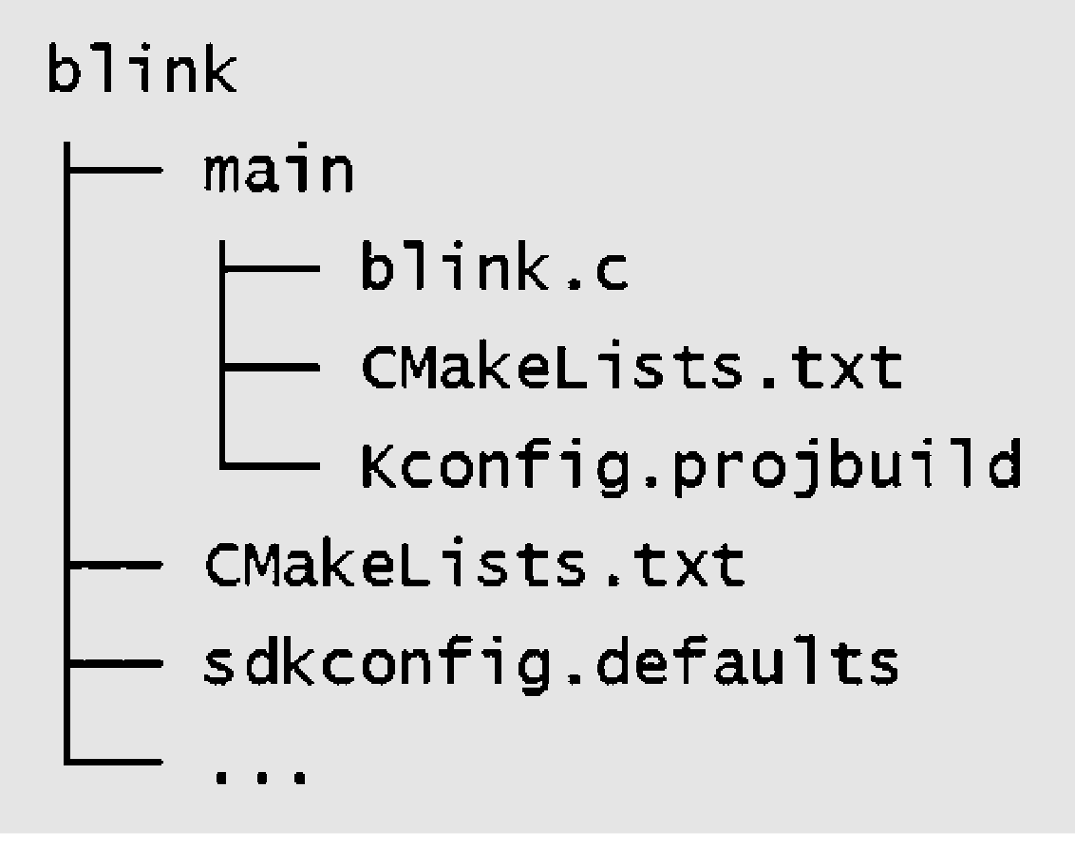
\includegraphics[width=0.6\textwidth]{D4Z/4-16}
    \caption{Automatic addition of environment variables in Windows system}
    \label{Automatic addition of environment variables in Windows system}
\end{figure}

For Windows systems, you can directly find and open ESP-IDF 4.3 CMD or ESP-IDF 4.3 PowerShell in the program list. After the terminal is opened, the environment variables will be automatically added, as shown in Figure \ref{Automatic addition of environment variables in Windows system}.

\subsubsection{2. Navigate to the root directory of the \texttt{blink} project}
Before compiling the project, navigate to the root directory of the project. To do this, use the command \verb|cd examples/get-started/blink|.

\subsubsection{3. Set the compilation target to ESP32-C3}
Use the command \verb|idf.py set-target esp32c3| to set the compilation target to ESP32-C3, as shown in Figure \ref{Set the compilation target to ESP32-C3}. If this step is skipped, the compilation target defaults to ESP32.

\begin{figure}[h!]
    \Centering
    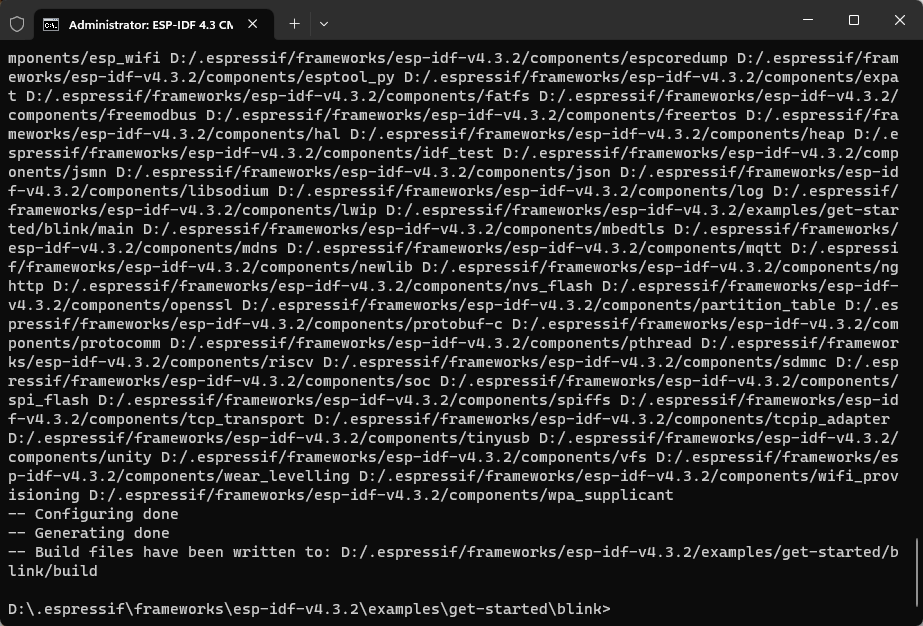
\includegraphics[width=0.63\textwidth]{D4Z/4-17}
    \caption{Set the compilation target to ESP32-C3}
    \label{Set the compilation target to ESP32-C3}
\end{figure}

\subsubsection{4. Configure GPIOs}
Use the command \verb|idf.py menuconfig| to enter the configuration interface. Navigate using the up/down keys and press Enter key to enter the \verb|Example Configuration|. Enter a number to change the GPIO to the specified pin, as shown in Figure 
\ref{Configure GPIO using menuconfig}. Save the configuration by following the prompts.

\begin{figure}[h!]
    \Centering
    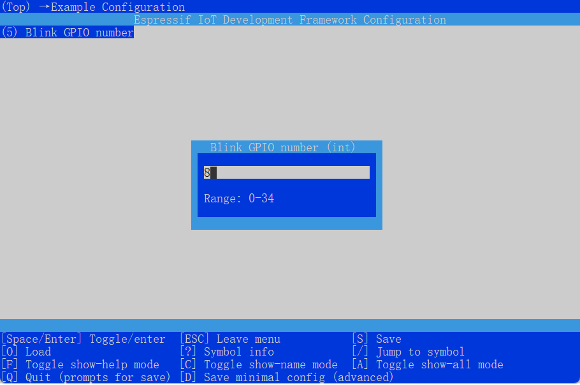
\includegraphics[width=0.55\textwidth]{D4Z/4-18}
    \caption{Configure GPIO using \texttt{menuconfig}}
    \label{Configure GPIO using menuconfig}
\end{figure}

\subsubsection{5. Build the code}
Use the command \verb|idf.py build| to build the code. The code building process is shown in Figure \ref{Code compilation process}. Relevant prompts and flash commands will be printed once the build is complete, as shown in Figure \ref{Prompt after code compilation is complete}.

\begin{figure}[h!]
    \Centering
    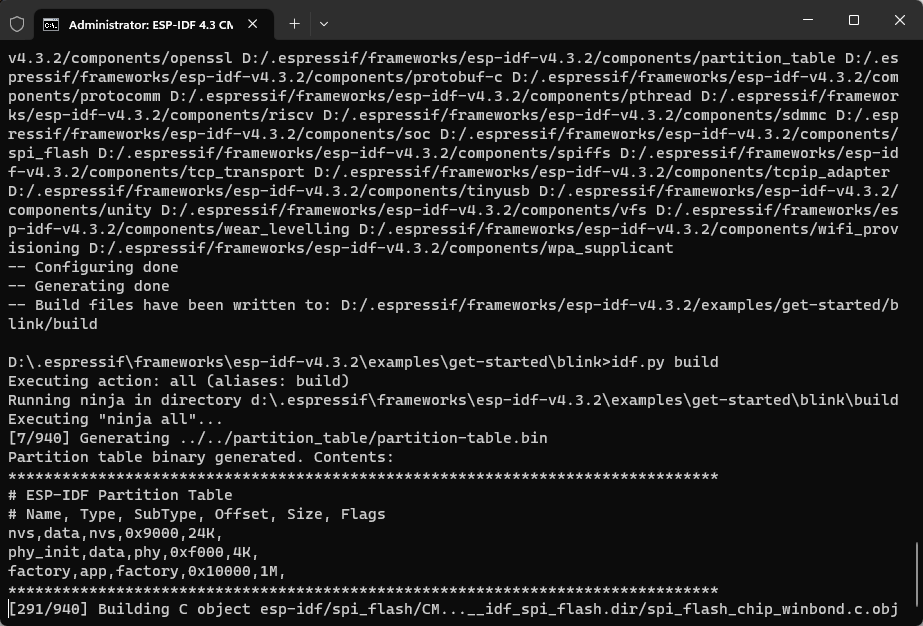
\includegraphics[width=0.55\textwidth]{D4Z/4-19}
    \caption{Code compilation process}
    \label{Code compilation process}
\end{figure}

\begin{figure}[h!]
    \Centering
    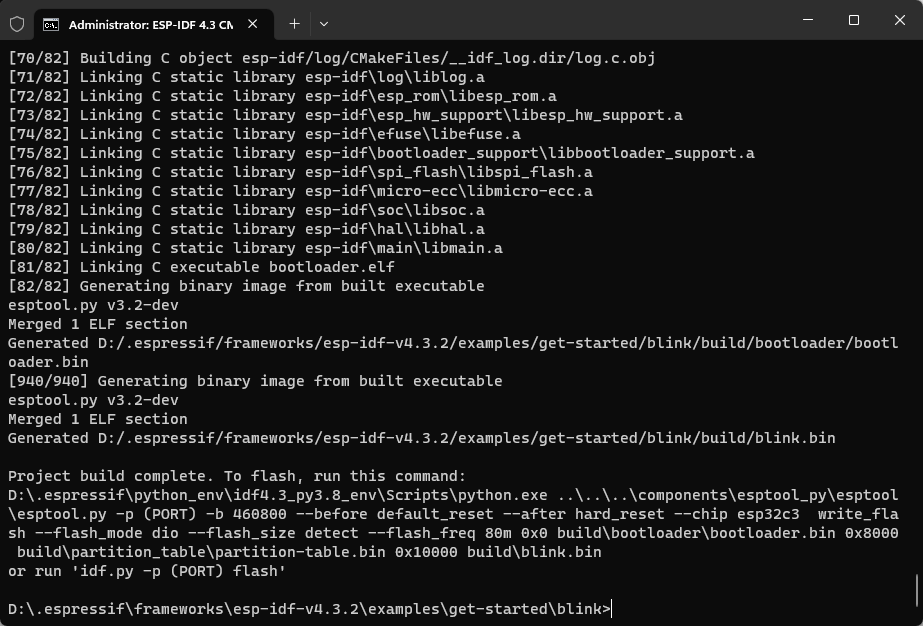
\includegraphics[width=0.55\textwidth]{D4Z/4-20}
    \caption{Prompt after code compilation is complete}
    \label{Prompt after code compilation is complete}
\end{figure}

\subsection{Flashing the Blink Program}
For Linux systems, connect the ESP32-C3 to the computer via USB-UART chip (such as CP2102), and use the command \verb|ls /dev/ttyUSB*| to view the serial port number. If the current serial port number printed is \verb|/dev/ttyUSB0|, use the command \verb|idf.py -p /dev|\\ \verb|/ttyUSB0 flash| to flash the program onto the ESP32-C3.

For Mac systems, connect the ESP32-C3 to the computer via USB-UART chip (such as CP2102), and use the command \verb|ls /dev/cu.*| to view the serial port number. If the current serial port number printed is \verb|/dev/cu.SLAB_USBtoUART|, use the command \verb|idf.py |\\ \verb|-p /dev/cu.SLAB_USBtoUART flash| to flash the program onto the ESP32-C3.

For Windows systems, connect the ESP32-C3 to the computer via USB-UART chip (such as CP2102), and view the serial port number through the device manager. If the current serial port number is \verb|COM5|, use the command \verb|idf.py -p COM5 flash| to flash the program onto the ESP32-C3.

After the flashing process is completed, you will see a prompt as shown in Figure \ref{Prompt in the console after flashing is completed} in the console. When the following log appears, the code will start executing, and the LED on the development board will start flashing.

\begin{codebloc}
\begin{tabular}{d}
Hard resetting via RTS pin...

Done
\end{tabular}
\end{codebloc}

\begin{figure}[h!]
    \Centering
    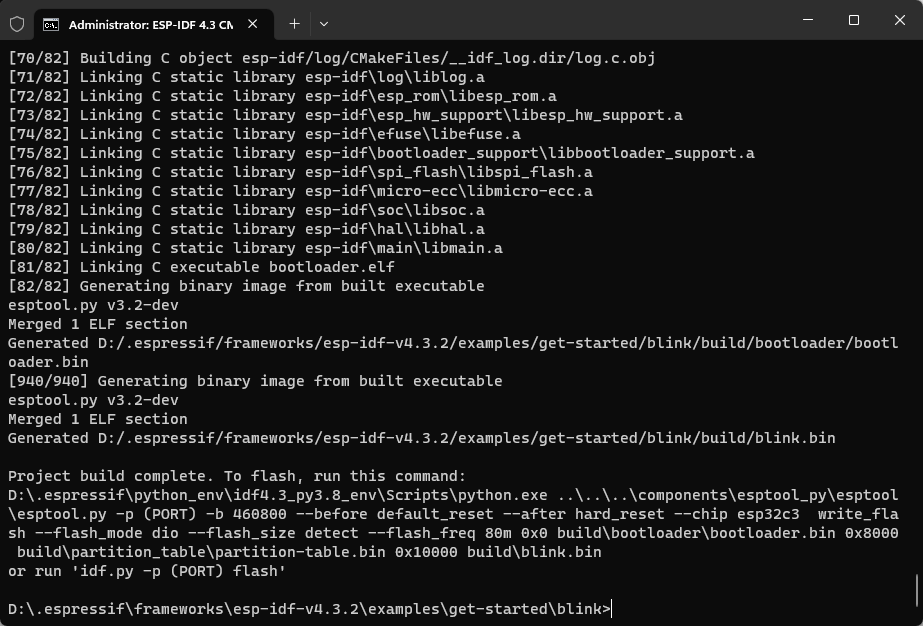
\includegraphics[width=0.7\textwidth]{D4Z/4-21}
    \caption{Prompt in the console after flashing is completed}
    \label{Prompt in the console after flashing is completed}
\end{figure}

\subsection{Serial Port Log Analysis of the Blink Program}
Once the firmware compilation and download are completed, navigate to the project folder, and run the command \verb|idf.py monitor|. This will open a monitor with coloured font. The monitor will output the serial port log of the target ESP32-C3. The content is divided into three parts by default: \textbf{first-level bootloader information}, \textbf{second-level bootloader information}, and \textbf{user program output}. During the output of log, you can press the \verb|Ctrl+]| key combination to exit the log output.

\begin{codebloc}
\begin{tabular}{d}
\vspace{2pt}
\begin{verbatim}
ESP-ROM:esp32c3-api1-20210207
Build:Feb  7 2021
rst:0x1 (POWERON),boot:0xc (SPI_FAST_FLASH_BOOT)
SPIWP:0xee
mode:DIO, clock div:1
load:0x3fcd6100,len:0x1798
load:0x403ce000,len:0x8dc
load:0x403d0000,len:0x2984
\end{verbatim}
\verb|entry 0x403ce000|
\end{tabular}
\end{codebloc}

\subsubsection{First-level bootloader information}
By default, the first-level bootloader information is output from UART and cannot be turned off through configuration in ESP-IDF version 4.3.2. This information includes the ROM code version information fixed internally in the chip. Different chips in the same series may have different ROM code versions due to ROM repairs and feature expansions. It also includes the reason for the chip restart, such as \verb|rst:0x1| indicating power-on restart of the chip, \verb|rst:0x3| indicating software-triggered restart, \verb|rst:0x4| indicating software exception restart, etc. You can use this information to assess the status of the chip. Additionally, it provides details about the chip’s boot mode, such as \verb|boot:0xc| indicating SPI Flash Boot mode (normal operation mode, in which the code in flash is loaded and executed), and \verb|boot:0x4| indicating Flash Download mode, in which the content of flash can be erased and programmed.

\subsubsection{Second-level bootloader information}
The output of second-level bootloader information can be disabled by setting \verb|menuconfig|\\ \verb|(Top) → Bootloader config → Bootloader log verbosity| to \verb|No output|.

This information mainly includes the ESP-IDF version, flash operating mode and speed, system partition and stack allocation, as well as the application name and version.

\begin{codebloc}
\begin{tabular}{d}
\vspace{2pt}
\begin{verbatim}
I (30) boot: ESP-IDF v4.3.2-1-g887e7c0c73-dirty 2nd stage bootloader
I (30) boot: compile time 18:27:35
I (30) boot: chip revision: 3
\end{verbatim}
\verb|I (34) boot.esp32c3: SPI Speed      : 80MHz|
\end{tabular}
\end{codebloc}

\begin{codebloc}
\begin{tabular}{d}
\vspace{2pt}
\begin{verbatim}
I (38) boot.esp32c3: SPI Mode       : DIO
I (43) boot.esp32c3: SPI Flash Size : 2MB
I (48) boot: Enabling RNG early entropy source...
I (53) boot: Partition Table:
I (57) boot: ## Label           Usage           Type ST Offset   Length
I (64) boot:  0 nvs             WiFi data       01 02 00009000 00006000
I (72) boot:  1 phy_init        RF data         01 01 0000f000 00001000
I (79) boot:  2 factory         factory app     00 00 00010000 00100000
I (86) boot: End of partition table
\end{verbatim}
\fontsize{9.5pt}{10pt}\selectfont
\begin{verbatim}
I (91) esp_image: segment 0: paddr=00010020 vaddr=3c020020 size=06058h (24664) map
I (103) esp_image: segment 1: paddr=00016080 vaddr=3fc89c00 size=01a88h (6792) load
I (109) esp_image: segment 2: paddr=00017b10 vaddr=40380000 size=08508h (34056) load
I (122) esp_image: segment 3: paddr=00020020 vaddr=42000020 size=15c54h (89172) map
I (138) esp_image: segment 4: paddr=00035c7c vaddr=40388508 size=0157ch (5500) load
I (139) esp_image: segment 5: paddr=00037200 vaddr=50000000 size=00010h (16) load
\end{verbatim}
\footnotesize
\begin{verbatim}
I (147) boot: Loaded app from partition at offset 0x10000
I (150) boot: Disabling RNG early entropy source...
I (166) cpu_start: Pro cpu up.
I (179) cpu_start: Pro cpu start user code
I (179) cpu_start: cpu freq: 160000000
I (179) cpu_start: Application information:
I (182) cpu_start: Project name:   blink
I (186) cpu_start: App version:    v4.3.2-1-g887e7c0c73-dirty
I (193) cpu_start: Compile time:   Jan 26 2022 18:27:31
I (199) cpu_start: ELF file SHA256:  dadcae8e7bb964ab...
I (205) cpu_start: ESP-IDF:         v4.3.2-1-g887e7c0c73-dirty
I (212) heap_init: Initializing. RAM available for dynamic allocation:
I (219) heap_init: At 3FC8C4D0 len 00033B30 (206 KiB): DRAM
I (225) heap_init: At 3FCC0000 len 0001F060 (124 KiB): STACK/DRAM
I (232) heap_init: At 50000010 len 00001FF0 (7 KiB): RTCRAM
I (238) spi_flash: detected chip: generic
I (243) spi_flash: flash io: dio
W (247) spi_flash: Detected size(4096k) larger than the size in the binary image 
header(2048k). Using the size in the binary image header.
I (260) sleep: Configure to isolate all GPIO pins in sleep state
I (267) sleep: Enable automatic switching of GPIO sleep configuration
\end{verbatim}
\verb|I (274) cpu_start: Starting scheduler.|
\end{tabular}
\end{codebloc}

\subsubsection{User program output}
The user program output includes all information that is printed using the \verb|printf()| function, which is the standard output function in the C language, or the \verb|ESP_LOG()| function, which is a custom output function provided by ESP-IDF. It is recommended to use \verb|ESP_LOG()| because it allows you to specify the log level for better organisation and filtering of logs.

You can configure which logs above a certain level are output through \verb|menuconfig(Top) |\\ \verb|→ Component config → Log output|. This allows you to control the verbosity of the logs and customise the level of detail that is displayed during runtime.

\begin{codebloc}
\begin{tabular}{d}
\vspace{2pt}
\begin{verbatim}
I (278) gpio: GPIO[5]| InputEn: 0| OutfgputEn: 0| OpenDrain: 0| Pullup: 1| 
Pulldown: 0| Intr:0 
Turning off the LED
Turning on the LED
Turning off the LED
\end{verbatim}
\verb|Turning on the LED|
\end{tabular}
\end{codebloc}

In addition to log output, \verb|idf.py monitor| can also parse system exceptions and trace software errors. For example, when the application crashes, the following register dump and traceback information will be generated:

\begin{codebloc}
\begin{tabular}{d}
\vspace{2pt}
\begin{verbatim}
Guru Meditation Error of type StoreProhibited occurred on core 0. Exception was 
unhandled.
Register dump:
PC  : 0x400f360d  PS    : 0x00060330  A0    : 0x800dbf56  A1    : 0x3ffb7e00
A2  : 0x3ffb136c  A3    : 0x00000005  A4    : 0x00000000  A5    : 0x00000000
A6  : 0x00000000  A7    : 0x00000080  A8    : 0x00000000  A9    : 0x3ffb7dd0
A10 : 0x00000003  A11   : 0x00060f23  A12   : 0x00060f20  A13   : 0x3ffba6d0
A14 : 0x00000047  A15   : 0x0000000f  SAR   : 0x00000019  EXCCAUSE  : 0x0000001d
EXCVADDR: 0x00000000  LBEG : 0x4000c46c  LEND : 0x4000c477  LCOUNT  : 0x00000000

Backtrace: 0x400f360d:0x3ffb7e00 0x400dbf56:0x3ffb7e20 0x400dbf5e:0x3ffb7e40 
\end{verbatim}
\verb|0x400dbf82:0x3ffb7e60 0x400d071d:0x3ffb7e90|
\end{tabular}
\end{codebloc}

Based on the register address, the IDF monitor will query the compiled \verb|ELF| file and trace the code call process when the application crashes, outputting the function call information to the monitor:

\begin{codebloc}
\begin{tabular}{d}
\vspace{2pt}
\begin{verbatim}
Guru Meditation Error of type StoreProhibited occurred on core 0. Exception was 
unhandled.
Register dump:
PC  : 0x400f360d  PS    : 0x00060330  A0    : 0x800dbf56  A1    : 0x3ffb7e00
0x400f360d: do_something_to_crash at /home/gus/esp/32/idf/examples/get-started/
hello_world/main/./hello_world_main.c:57
(inlined by) inner_dont_crash at /home/gus/esp/32/idf/examples/get-started/hello
_world/main/./hello_world_main.c:52
A2  : 0x3ffb136c  A3    : 0x00000005  A4    : 0x00000000  A5    : 0x00000000
A6  : 0x00000000  A7    : 0x00000080  A8    : 0x00000000  A9    : 0x3ffb7dd0
A10 : 0x00000003  A11   : 0x00060f23  A12   : 0x00060f20  A13   : 0x3ffba6d0
A14 : 0x00000047  A15   : 0x0000000f  SAR   : 0x00000019  EXCCAUSE  : 0x0000001d
EXCVADDR: 0x00000000  LBEG : 0x4000c46c  LEND : 0x4000c477  LCOUNT  : 0x00000000

Backtrace: 0x400f360d:0x3ffb7e00 0x400dbf56:0x3ffb7e20 0x400dbf5e:0x3ffb7e40 
0x400dbf82:0x3ffb7e60 0x400d071d:0x3ffb7e90
0x400f360d: do_something_to_crash at /home/gus/esp/32/idf/examples/get-started/ 
\end{verbatim}
\verb|hello_world/main/./hello_world_main.c:57|
\end{tabular}
\end{codebloc}

\begin{codebloc}
\begin{tabular}{d}
\vspace{2pt}
\begin{verbatim}
(inlined by) inner_dont_crash at /home/gus/esp/32/idf/examples/get-started/hello
_world/main/./hello_world_main.c:52
0x400dbf56: still_dont_crash at /home/gus/esp/32/idf/examples/get-started/hello
_world/main/./hello_world_main.c:47
0x400dbf5e: dont_crash at /home/gus/esp/32/idf/examples/get-started/hello_world/
main/./hello_world_main.c:42
0x400dbf82: app_main at /home/gus/esp/32/idf/examples/get-started/hello_world/
main/./hello_world_main.c:33
\end{verbatim}
\verb|0x400d071d: main_task at /home/gus/esp/32/idf/components/esp32/./cpu_start.c:254|
\end{tabular}
\end{codebloc}

The trace information of the monitor shows that the application crashes in the function \verb|do_something_to_crash()|, which is called by the function \verb|app_main() → dont_|\\ \verb|crash() → still_dont_crash() → inner_dont_crash() → do_something|\\ \verb|_to_crash()|. Based on this, the input/output parameters of each link can be checked to determine the cause of the crash.

\section{Summary}
In this chapter, we have covered the setup of the official software development environment, ESP-IDF, for ESP32-C3. We have introduced the code resources and file structure of ESP-IDF and provided a demonstration of the ESP-IDF project structure, compilation system, and related development tools using a simple example.

By following the instructions in this chapter, you can start developing with ESP-IDF for simple projects. However, for more specific and advanced compilation requirements, it is recommended to refer to both the ESP-IDF official documentation and the CMake official documentation.

\end{document}